
%packages
\usepackage{natbib}
\usepackage{amsmath}
\usepackage{amsthm}
\usepackage{mathtools}
\usepackage{mdframed}
\usepackage{subfigure}
\usepackage{booktabs}
% \usepackage{hyperref}
\usepackage{subfigure}
\usepackage{siunitx} % Provides the \SI{}{} and \si{} command for typesetting SI units
\usepackage{graphicx} % Required for the inclusion of images
% \usepackage{natbib} % Required to change bibliography style to APA
\usepackage{datetime}
\usepackage{lscape}
\usepackage{algorithm}
\usepackage{algorithmic}
\usepackage{xspace}
\usepackage[english]{babel} % English language/hyphenation
\usepackage{proof}
\usepackage{booktabs} % Top and bottom rules for tables
\usepackage[colorlinks, allcolors = blue,]{hyperref}
\usepackage{accents}
\usepackage{amsfonts}
\usepackage{stmaryrd}
\usepackage{amsmath,amsthm,amssymb,latexsym} 
\usepackage{microtype}
\usepackage{graphicx}
\usepackage{subfigure}
\usepackage{booktabs} % for professional tables
\usepackage{hyperref}
\usepackage{icml2019}
\usepackage{lipsum}

\usepackage{authblk}


%new commands
\newcommand{\theHalgorithm}{\arabic{algorithm}}
\newtheorem{definition}{Definition}
\usepackage{cancel}
\usepackage[normalem]{ulem}
\newcommand{\dataobs}{\textbf{x}}
\newcommand{\adj}[2]{\textbf{adj}(#1,#2)}
\newcommand{\candidateset}{\mathcal{R}_{\textup{post}}}
\newcommand{\bprior}{\boldsymbol{\beta}_{\textup{prior}}}
\newcommand{\bysinfer}{\mathsf{Infer}}
\newcommand{\betad}{\mathsf{Beta}}
\newcommand{\betaf}{\textup{B}}
\newcommand{\mbetaf}{\boldsymbol{\textup{B}}}
\newcommand{\vtheta}{\boldsymbol{\theta}}
\newcommand{\valpha}{\boldsymbol{\alpha}}
\newcommand{\vbeta}{\boldsymbol{\beta}}
\newcommand{\lapmech}{\mathsf{LSDim}}
\newcommand{\ilapmech}{\mathsf{LSHist}}
\newcommand{\binomial}[2]{\mathsf{Bin}(#1, #2)}
\newcommand{\multinomial}[2]{\mathsf{Mult}(#1, #2)}
\newcommand{\expmech}{\mathsf{EHD}}
\newcommand{\hexpmech}{\mathsf{EHDS}}
\newcommand{\lexpmech}{\mathsf{EHDL}}
\newcommand{\hexpmechd}{\mathsf{expMech}^{D}_{\hellinger}}
\newcommand{\privinfer}{\mathsf{PrivInfer}}
\newcommand{\hlg}{\mathsf{H}}
\newcommand{\dirichlet}[1]{\mathsf{Dir}(#1)}
\newcommand{\alphas}{\boldsymbol{\alpha}}
\newcommand{\xis}{\boldsymbol{\xi}}
\newcommand{\iverson}[1]{[#1]}
\newcommand{\datauni}{\mathcal{X}}
\newcommand{\hellinger}{\mathcal{H}}
\newcommand{\ux}[1]{u(\textbf{x}, {#1})}
\newcommand{\uxadj}[1]{u(\textbf{x}', {#1})}
\newcommand{\cardinality}[2]{\mathcal{C}^{#1}_{#2}}
\newcommand{\range}{\mathcal{O}}
\newcommand{\nomalizer}[1]{\sum\limits_{r'\in \mathcal{R}_{\textup{post}}} \exp \big(\frac{-\epsilon\cdot \mathcal{H} (\mathsf{BI}(#1),r')}{4 \cdot S(#1)}\big)}

\newcommand{\unomalizer}[1]{\sum\limits_{r'\in \mathcal{R}_{\textup{post}}} \exp \big(\frac{-\epsilon\cdot u(#1, r')}{4 \cdot S(#1)}\big)}


\newcommand{\hexpmechPr}[2]{\underset{z \thicksim \hexpmech(#1)}{\Pr}\left[ #2 \right]}
\newcommand{\lapmechPr}[2]{\underset{z \thicksim \lapmech(#1)}{\Pr}\left[ #2 \right]}

\newcommand{\ilapmechPr}[2]{\underset{
{z \thicksim \ilapmech(#1)}
}{\Pr}\left[ #2 \right]}

\newtheorem{thm}{Theorem}[section]

\newtheorem{lem}{Lemma}[section]

\newtheorem{assert}{Assertion}[lem]
\newcommand{\lap}[2]{\mathsf{Lap}(#1, #2)}
\newcommand{\todo}[1]{{\footnotesize \color{red}\textbf{[[ #1 ]]}}}

\title{\textbf{Notes of DP - Bayesian Inference}\\}
% \author{Jiawen \textsc{Liu}}
\date{\vspace{-10ex}}

\begin{document}
\maketitle

\section{Bayesian Inference Based on Dirichlet-Bernoulli Distribution}
\label{sec_bayesInfer}
In the Bayesian inference, first there is a prior distribution $\pi(\xis)$ to present our belief about parameter $\xis$. Then, we get some observed data $x$ sizing $n$, and produce a posterior distribution $Pr(\xis | x)$. The Bayesian inference is based on the Bayes' rule to calculate the posterior distribution:
\begin{equation*}
Pr(\xis | x) = \frac{Pr(x | \xis) \pi(\xis)}{Pr(x)}
\end{equation*}
It is denoted as $\bysinfer(x,\pi(\xis))$ taking an observed data set $x \in \mathcal{X}^n$ and a prior distribution $\pi(\xis)$ as input, outputting a posterior distribution of the parameter $\alphas$. For conciseness, when prior is given, we use $\bysinfer(x)$. $n$ is the size of the observed data size.

In our inference algorithm, we take a Dirichlet distribution as prior belief for the parameters, $\dirichlet(\alphas)$, where $\pi(\xis) = \dirichlet(\xis | \alphas) = \frac{\prod_{i = 1}^{m}\xi_i^{\alpha_i}}{B(\alphas)}$, and the Bernoulli distribution as the statistic model for $Pr(x | \alphas)$. $m$ is the order of the Dirichlet distribution.

We give a inference process based on a concrete example, where we throw an irregular $m$ sides dice. We want to infer the probability of getting each side $\xis$. We get a observed data set $\{s_{k_1}, s_{k_2}, \cdots, s_{k_n}\}$ by throwing the dice $n$ times, where $k_i \in \{1,2,\cdots, m\}$ denotes the side we get when we throw the dice the $i^{th}$ time. The posterior distribution is still a Dirichlet distribution with parameters $(\alpha_1 + n_1, \alpha_2 + n_2, \cdots, \alpha_m + n_m)$, where $n_i$ is the appearance time of the side $i$ in total.

In the case that $m = 2$, it is reduced to a Beta distribution $\betad(\alpha, \beta)$. The $m$ side dice change into a irregular coin with side $A$ and side $B$. The posterior is computed as $(\alpha + n_1, \beta + n_0)$, where $n_1$ is the appearance time of side $A$ in the observed data set and $n_0$ is the appearance time of the other side.



\section{Algorithm Setting up}
\label{sec_setup}
For now, we already have a prior distribution $\pi(\xis)$, an observed data set $x$.

\subsection{Exponential Mechanism with Global Sensitivity}
\label{subsec_emgs}

% \subsubsection{Mechanism Set up}

In exponential mechanism, candidate set $\mathcal{R}$ can be obtained by enumerating $y \in \mathcal{X}^n$, i.e.
\begin{equation*}
\mathcal{R} = \{\bysinfer(y)\ |\ y \in \mathcal{X}^n\}.
\end{equation*}

Hellinger distance $\hlg$ is used here to score these candidates. The utility function:
\begin{equation}
\label{equ_utility}
u(x,r) = -\hlg(\bysinfer(x), r); r \in \mathcal{R}.
\end{equation}

Exponential mechanism with global sensitivity selects and outputs a candidate $r \in \mathcal{R}$ with probability proportional to $exp(\frac{\epsilon u(x,r)}{2 \Delta_{g}u})$:
\begin{equation*}
P[r] = \frac
{exp(\frac{\epsilon u(x,r)}{2 \Delta_{g}u})}
{\Sigma_{r' \in \mathcal{R}}\ exp(\frac{\epsilon u(x,r')}{2 \Delta_{g}u})},
\end{equation*}
where global sensitivity is calculated by:
\begin{equation*}
\Delta_{g}u = 
\max_{\{|x',y'| \leq 1;x',y'\in \mathcal{X}^n\}}\max_{\{r\in \mathcal{R}\}}
|\hlg(\bysinfer(x'), r) - \hlg(\bysinfer(y'), r)|
\end{equation*}

The basic exponential mechanism is $\epsilon -$differential privacy\cite{dwork2014algorithmic}.

% We use probability proportional to $exp(\frac{\epsilon u(x,r)}{\Delta_{g}u})$ rather than $exp(\frac{\epsilon u(x,r)}{2 \Delta_{g}u})$. Since $\hlg$ is monotonic, i.e. our utility function is monotonic. 

% \subsubsection{Security Analysis}
% It can be proved that exponential mechanism with global sensitivity is $\epsilon$-differentially private. We denote the $\bysinfer$ with privacy mechanism as $\privinfer$. For adjacent data set $||x,y||_1 = 1$:
% \begin{equation*}
% \begin{split}
% \frac{P[\privinfer(x,u,R) = r]}{P[\privinfer(y,u,R) = r]}
% & =\frac
% {\frac
% {exp(\frac{\epsilon u(x,r)}{2 \Delta_{g}u})}
% {\Sigma_{r' \in R}\ exp(\frac{\epsilon u(x,r')}{2 \Delta_{g}u})}}
% {\frac
% {exp(\frac{\epsilon u(y,r)}{2 \Delta_{g}u})}
% {\Sigma_{r' \in R}\ exp(\frac{\epsilon u(y,r')}{2 \Delta_{g}u})}} \\
% & = \left(\frac
% {exp(\frac{\epsilon u(x,r)}{2 \Delta_{g}u})}
% {exp(\frac{\epsilon u(y,r)}{2 \Delta_{g}u})}
% \right)
% \cdot
% \left(\frac
% {\sum\limits_{r' \in R}\ exp(\frac{\epsilon u(y,r')}{2 \Delta_{g}u})}
% {\sum\limits_{r' \in R}\ exp(\frac{\epsilon u(x,r')}{2 \Delta_{g}u})}
% \right)\\
% & = exp\left(\frac
% {\epsilon (u(x,r) - u(y,r))}
% {2 \Delta_{g}u}
% \right)
% \cdot
% \left(\frac
% {\sum\limits_{r' \in R}\ exp(\frac{\epsilon u(y,r')}{2 \Delta_{g}u})}
% {\sum\limits_{r' \in R}\ exp(\frac{\epsilon u(x,r')}{2 \Delta_{g}u})}
% \right)\\
% & \leq
% exp(\frac{\epsilon}{2}) \cdot exp(\frac{\epsilon}{2}) \cdot
% \left(\frac
% {\sum\limits_{r' \in R}\ exp(\frac{\epsilon u(x,r')}{2 \Delta_{g}u})}
% {\sum\limits_{r' \in R}\ exp(\frac{\epsilon u(x,r')}{2 \Delta_{g}u})}
% \right)\\
% & = exp(\epsilon).
% \end{split}
% \end{equation*}

% Then, $\frac{P[\privinfer(x,u,R) = r]}{P[\privinfer(y,u,R) = r]} \geq exp(-\epsilon)$ can be obtained by symmetry.


\subsection{Exponential Mechanism with Local Sensitivity}
\label{subsec_emls}
% \subsubsection{Mechanism Set up}
Exponential mechanism with local sensitivity share the same candidate set and utility function as it with global sensitivity. This outputs a candidate $r \in \mathcal{R}$ with probability proportional to $exp(\frac{\epsilon u(x,r)}{2 \Delta_{l}u})$:
\begin{equation*}
P[r] = \frac
{exp(\frac{\epsilon u(x,r)}{2 \Delta_{l}u})}
{\Sigma_{r' \in \mathcal{R}}\ exp(\frac{\epsilon u(x,r')}{2 \Delta_{l}u})},
\end{equation*}

where local sensitivity is calculated by:

\begin{equation*}
\Delta_{l}u(x) = 
\max_{\{|x,y'| \leq 1;y'\in \mathcal{X}^n\}}\max_{\{r\in \mathcal{R}\}}.
\hlg(\bysinfer(x), r) - \hlg(\bysinfer(y'), r)|
\end{equation*}

The exponential mechanism with local sensitivity is non differential privacy\cite{dwork2014algorithmic}.


\subsection{Exponential Mechanism with Smooth Sensitivity}
\label{sec_smoo}

\subsubsection{Algorithm Setting up}
We define a new mechanism $\hexpmech(x)$
which is similar to the exponential mechanism where we use
$\mathcal{R}$ as the set $\betaset$ of beta distributions with integer parameters
summing up to $n+2$, as scoring function we use the Hellinger distance
from $\bysinfer(x)$, i.e. $\hlg(\bysinfer(x),-)$, and we 
calibrate the noise to the smooth sensitivity~\cite{nissim2007smooth}. The
only difference is in the sensitivity part, since now we use the
smooth sensitivity.

\begin{definition} The mechanism $\hexpmech(x)$ outputs a candidate $r \in \betaset$ with probability
\begin{equation*}
\underset{z \thicksim \hexpmech(x)}{Pr}[z=r] = \frac
{exp(\frac{-\epsilon\hlg(\bysinfer(x),r)}{2 S_\beta(x)})}
{\Sigma_{r' \in R}\ exp(\frac{-\epsilon \hlg(\bysinfer(x),r')}{2 S_\beta(x)})},
\end{equation*}
where $s_\beta(x)$ is the smooth sensitivity of $\hlg(\bysinfer(x),-)$, calculated by:
\begin{equation*}
S_{\beta}(x) = \max(\Delta_{l}\hlg(\bysinfer(x),-), \max_{y \neq x; y \in D^{n}}(\Delta_{l}\hlg(\bysinfer(y),-)\cdot e^{-\beta d(x,y)})),
\end{equation*}
where $d$ is the Hamming distance between two datasets, and $\beta =
\beta(\epsilon, \delta)$ is a function of $\epsilon$ and $\delta$. 
\end{definition}


In what follows, we will use a correspondence between the probability
 $\underset{z \thicksim \hexpmech(x)}{Pr}[z = r]$ of every
 $r\in\betaset$ and the probability 
 $\underset{z \thicksim \hexpmech(x)}{Pr}[\hlg(\bysinfer(x),z) =
 \hlg(\bysinfer(x),r)]$ for the utility score for $r$. In particular, for every
 $r\in\betaset$ we have:
$$
\underset{z \thicksim \hexpmech(x)}{Pr}[z = r]=
\frac{1}{2}\Big (\underset{z \thicksim \hexpmech(x)}{Pr}[\hlg(\bysinfer(x),z) =
 \hlg(\bysinfer(x),r)]\Big )
$$
To see this, it is enough to notice that: $\underset{z \thicksim \hexpmech(x)}{Pr}[z = r]$ is proportional too $\hlg(\bysinfer(x),r)$, i.e., $u(x,z)$. We can derive, if $u(r,x) = u(r',x)$ then $\underset{z \thicksim \hexpmech(x)}{Pr}[z = r] = \underset{z \thicksim \hexpmech(x)}{Pr}[z = r']$. We assume the number of candidates $z \in \mathcal{R}$ that satisfy $u(z,x) = u(r,x)$ is $|r|$, we have  $\underset{z \thicksim \hexpmech(x)}{Pr}[u(z,x) = u(r,x)] = |r| \underset{z \thicksim \hexpmech(x)}{Pr}[z = r]$. Because Hellinger distance  $\hlg(\bysinfer(x),z)$ is axial symmetry, where the $\bysinfer(x)$ is the symmetry axis. It can be infer that $|z| = 2$ for any candidates, apart from the true output, i.e., $\underset{z \thicksim \hexpmech(x)}{Pr}[u(z,x) = u(r,x)] = 2 \underset{z \thicksim \hexpmech(x)}{Pr}[z = r]$. This parameter can be eliminate in both sides in proof.

In our private Bayesian inference mechanism, we set the $\beta$ as $\ln(1 - \frac{\epsilon}{2 \ln (\frac{\delta}{2 (n + 1)})})$. 


\subsubsection{Sliding Property of Exponential Mechanism}
\begin{lem}
Consider the exponential mechanism  $\sexpmech(x,u,\mathcal{R})$
calibrated on the smooth sensitivity. Let $\lambda = f(\epsilon,
\delta)$, $\epsilon\geq 0$ and $|\delta| < 1$. Then, the following \emph{sliding property} holds:
\begin{equation*}
\underset{r \thicksim \hexpmech(x)}{Pr}[u(r,x) = \hat{s}]
\leq
e^{\frac{\epsilon}{2}} \underset{r \thicksim \hexpmech(x)}{Pr}[u(r,x) = (\Delta + \hat{s})] + \frac{\delta}{2},
\end{equation*}

\end{lem}

\begin{proof}

We denote the normalizer of the probability mass in $\hexpmech(x)$: $\sum_{r' \in \mathcal{R}}exp(\frac{\epsilon u(r',x)}{2 S(x)})$ as $NL(x)$:
\begin{equation*}
\begin{split}
LHS 
  = \underset{r \thicksim \hexpmech(x)}{Pr}[u(r,x) = \hat{s}]
& = \frac{exp(\frac{\epsilon \hat{s}}{2 S(x)})}{NL(x)}\\
& = \frac{exp(\frac{\epsilon (\hat{s} + \Delta - \Delta)}{2 S(x)})}{NL(x)}\\
& = \frac{exp(\frac{\epsilon (\hat{s} + \Delta)}{2 S(x)} + \frac{- \epsilon \Delta}{2 S(x)})}{NL(x)}\\
& = \frac{exp(\frac{\epsilon (\hat{s} + \Delta)}{2 S(x)})}{NL(x)} \cdot e^{\frac{- \epsilon \Delta}{2 S(x)})}.\\
\end{split}
\end{equation*}

By bounding the $\Delta \geq -S(x)$, we can get:

\begin{equation*}
\begin{split}
\frac{exp(\frac{\epsilon (\hat{s} + \Delta)}{2 S(x)})}{NL(x)} \cdot e^{\frac{- \epsilon \Delta}{2 S(x)}}
& \leq \frac{exp(\frac{\epsilon (\hat{s} + \Delta)}{2 S(x)})}{NL(x)} \cdot e^{\frac{\epsilon}{2}}\\
&  =  e^{\frac{\epsilon}{2}} \underset{z \thicksim \hexpmech(x)}{Pr}[u(r,x) = (\Delta + \hat{s})] \leq RHS\\
\end{split}
\end{equation*}

\end{proof}

\subsubsection{Dilation Property of Exponential Mechanism}
\begin{lem}
for any exponential mechanism $\hexpmech(x)$, $\lambda < |\beta|$, $\epsilon$, $|\delta| < 1$ and $\beta \leq \ln(1 - \frac{\epsilon}{2 \ln (\frac{\delta}{2 (n + 1)})})$, the dilation property holds:

\begin{equation*}
\underset{z \thicksim \hexpmech(x)}{Pr}[u(z,x) = c]
\leq
e^{\frac{\epsilon}{2}} \underset{z \thicksim \hexpmech(x)}{Pr}[u(z,x) = e^{\lambda} c] + \frac{\delta}{2},
\end{equation*}
where the sensitivity in mechanism is still smooth sensitivity as above.
\end{lem}

\begin{proof}

The sensitivity is always greater than 0, and our utility function $-\hlg(\bysinfer(x),z)$ is smaller than zero, i.e., $u(z,x) \leq 0$, we need to consider two cases where $\lambda < 0$, and $\lambda > 0$:

We set the $h(c) = Pr[u(\hexpmech(x)) = c] = 2\frac{exp(\frac{\epsilon z}{2 S(x)})}{NL(x)}$.

We first consider $\lambda < 0$. In this case, $1 < e ^ {\lambda}$, so the ratio $\frac{h(c)}{h(e^{\lambda}c)} = \frac{exp(\frac{\epsilon c}{2 S(x)})}{exp(\frac{\epsilon (c \cdot e^{\lambda})}{2 S(x)})}$ is at most $\frac{\epsilon}{2}$.

Next, we proof the dilation property for $\lambda > 0$, The ratio of $\frac{h(c)}{h(e^{\lambda}c)}$ is $\exp(\frac{\epsilon}{2} \cdot \frac{u(\hexpmech(x)) (1 - e^{\lambda})}{S(x)})$. Consider the event $G = \{ \hexpmech(x) : u(\hexpmech(x)) \leq \frac{S(x)}{(1 - e^{\lambda})}\}$. Under this event, the log-ratio above is at most $\frac{\epsilon}{2}$. The probability of $G$ under density $h(c)$ is $1 - \frac{\delta}{2}$. Thus, the probability of a given event $z$ is at most $Pr[c \cap G] + Pr[\overline{G}] \leq e^{\frac{\epsilon}{2}} Pr[e^{\lambda}c \cap G] + \frac{\delta}{2} \leq e^{\frac{\epsilon}{2}} Pr[e^{\lambda}c] + \frac{\delta}{2}$.\\


\textbf{Detail proof:}
\begin{itemize}

	\item $\lambda < 0$

		The left hand side will always be smaller than 0 and the right hand side greater than 0. This will always holds, i.e.
		\begin{equation*}
		\end{equation*}
	\item $\lambda > 0$


Because $\hat{s} = u(r)$ where $r \thicksim \hexpmech(x)$, we can substitute $\hat{s}$ with $u(\hexpmech(x))$. Then, what we need to proof under the case $\lambda > 0$ is:
\begin{equation*}
u(\hexpmech(x)) \leq \frac{S(x)}{(1 - e ^ {\lambda})}
\end{equation*}
By applying the accuracy property of exponential mechanism, we bound the probability that the equation holds with probability:
\begin{equation*}
\begin{split}
Pr[u(\hexpmech(x)) \leq \frac{S(x)}{(1 - e ^ {\lambda})}] 
& \leq \frac{|\mathcal{R}|exp(\frac{\epsilon S(x)}{(1 - e ^ {\lambda})}/2 S(x))}{|\mathcal{R}_{OPT}| exp(\epsilon OPT_{u(x)}/2 S(x))}\\
\end{split}
\end{equation*}

In our Bayesian Inference mechanism, the size of the candidate set $\mathcal{R}$ is equal to the size of observed data set plus 1, i.e., $n + 1$, and $OPT_{u(x)} = 0$, then we have:
\begin{equation*}
\begin{split}
Pr[u(\hexpmech(x)) \leq \frac{S(x)}{(1 - e ^ {\lambda})}] 
& = (n + 1)exp(\frac{\epsilon S(x)}{(1 - e ^ {\lambda})}/2 S(x))\\
& = (n + 1)exp(\frac{\epsilon}{2 (1 - e ^ {\lambda})})\\
\end{split}
\end{equation*}

When we set $\lambda \leq \ln(1 - \frac{\epsilon}{2 \ln (\frac{\delta}{2 (n + 1)})})$, it is easily to derive that $Pr[u(\hexpmech(x)) \leq \frac{S(x)}{(1 - e ^ {\lambda})}] \leq \frac{\delta}{2}$.

\end{itemize}

\end{proof}

\subsubsection{Privacy Analysis}
\begin{lem}
\label{lem_hexpmech_privacy}
$\hexpmech$ is $(\epsilon, \delta)$-differential privacy.
\end{lem}

\begin{proof}
of Lemma \ref{lem_hexpmech_privacy}: For all neighboring $x, y \in D^n$ and all sets $\mathcal{S}$, we need to show that:
\begin{equation*}
\underset{z \thicksim \hexpmech(x)}{Pr}[ z \in \mathcal{S}] \leq e^{\epsilon} \underset{z \thicksim \hexpmech(y)}{Pr}[z \in \mathcal{S}] + \delta. 
\end{equation*}
Given that $2\Big( \underset{z \thicksim \hexpmech(x)}{Pr}[ z \in \mathcal{S}]\Big) = \underset{z \thicksim \hexpmech(x)}{Pr}[ u(x,z) \in \mathcal{U}]$, let $\mathcal{U}_1 = \frac{u(y,z) - u(x,z)}{S(x)}$, $\mathcal{U}_2 = \mathcal{U} + \mathcal{U}_1$ and $\mathcal{U}_3 = \mathcal{U}_2 \cdot \frac{S(x)}{S(y)} \cdot \ln(\frac{NL(x)}{NL(y)})$. Then,

\begin{equation*}
\begin{split}
2\Big( \underset{z \thicksim \hexpmech(x)}{Pr}[ z \in \mathcal{S}]\Big)
& = \underset{z \thicksim \hexpmech(x)}{Pr}[ u(x,z) \in \mathcal{U}]\\
& \leq e^{\epsilon / 2} \cdot \underset{z \thicksim \hexpmech(x)}{Pr}[ u(x,z) \in \mathcal{U}_2]\\
& \leq e^{\epsilon} \cdot \underset{z \thicksim \hexpmech(x)}{Pr}[ u(x,z) \in \mathcal{U}_3] + e^{\epsilon/2} \cdot \frac{\delta'}{2}\\
& = e^{\epsilon} \cdot \underset{z \thicksim \hexpmech(y)}{Pr}[ u(y,z) \in \mathcal{U}] + \delta = 2\Big( e^{\epsilon} \cdot \underset{z \thicksim \hexpmech(x)}{Pr}[ z \in \mathcal{S}] \Big) + \delta\\
\end{split}
\end{equation*}

The first inequality holds by the sliding property, since the $\mathcal{U}_1 \geq -S(x)$. The second inequality holds by the dilation property, since $\frac{S(x)}{S(y)} \cdot \ln(\frac{NL(x)}{NL(y)}) \leq 1 - \frac{\epsilon}{2 \ln (\frac{\delta}{2 (n + 1)})}$.

\end{proof}

\section{Accuracy Analysis}
\subsection{Laplace Mechanism}
Fixing a data set $x$, we will sample noise $Lap_i = floor(Y)$ where $Y \sim Lap(\frac{2}{\epsilon})$. Since already had the accuracy bound based on the $l_1$ norm in Laplace mechanism:
\begin{equation*}
Pr[|Y| \geq t] = e^{- \frac{t \epsilon}{2}}.
\end{equation*}

So we have the probability $Pr[| Lap_i |] = Pr[| Lap_i | \leq |Y| < | Lap_i | + 1] = e^{- \frac{| Lap_i | \epsilon}{2}} - e^{- \frac{(| Lap_i | + 1) \epsilon}{2}}$.

When we are in the case of $m$ dimension Dirichlet distribution, we will add $(m-1)$ i.i.d. Laplace noises $\{| Lap_1 |, | Lap_2 |, \cdots, | Lap_{m-1} |\}$ to the output. Then the probability of each group of noises are calculated as $Pr[\{| Lap_1 |, | Lap_2 |, \cdots, | Lap_{m-1} |\}] = Pr[| Lap_1 | \leq |Y| < | Lap_1 | + 1] \times Pr[| Lap_2 | \leq |Y| < | Lap_2 | + 1] \times \cdots \times Pr[| Lap_{m-1} | \leq |Y| < | Lap_{m-1} | + 1] = (e^{- \frac{| Lap_1 | \epsilon}{2}} - e^{- \frac{(| Lap_1 | + 1) \epsilon}{2}}) \times (e^{- \frac{| Lap_2 | \epsilon}{2}} - e^{- \frac{(| Lap_2 | + 1) \epsilon}{2}}) \times \cdots \times (e^{- \frac{| Lap_{m-1} | \epsilon}{2}} - e^{- \frac{(| Lap_{m-1} | + 1) \epsilon}{2}})$.

% where $m$ is the order of the Dirichlet distribution. Then we have the accuracy bound based on $\hlg$ distance.
% \begin{equation*}
% \begin{split}
% Pr[||Lap(\bysinfer(x)) - \bysinfer(x)||_1 \geq m \ln (\frac{m}{\gamma}) \frac{2}{\epsilon}] & \leq Pr[m ||Lap(\bysinfer(x)) - \bysinfer(x)||_{\infty} \geq m \ln (\frac{m}{\gamma}) \frac{2}{\epsilon}]\\
% & = Pr[||Lap(\bysinfer(x)) - \bysinfer(x)||_{\infty} \geq \ln (\frac{m}{\gamma}) \frac{2}{\epsilon}]\\
% & = \gamma
% \end{split} 
% \end{equation*}


\subsection{Exponential Mechanism with Global Sensitivity}
Also, according to \cite{dwork2014algorithmic}, we already had the accuracy bound of exponential mechanism with global sensitivity as:
\begin{equation*}
\underset{z \thicksim \hexpmech(x)}{Pr}[ \hlg(\bysinfer(x), z) \geq c] \leq  \frac{|R| \exp{(\frac{- \epsilon c}{2 \Delta_g}})}{|R_{OPT}|\exp{(\frac{- \epsilon OPT_{\hlg(\bysinfer(x), z)}(x)}{2 \Delta_g})}},
\end{equation*}
where $|R|$ is the size of the candidate set. Since $OPT_{\hlg(\bysinfer(x), z)}(x) = 0$ and $|R_{OPT}| = 1$, we simplified accuracy bound here $\underset{z \thicksim \hexpmech(x)}{Pr}[ \hlg(\bysinfer(x), z) \geq c] \leq |R| \exp{(\frac{- \epsilon c}{2 \Delta_g}}),$


\subsection{Exponential Mechanism with Smooth Sensitivity}
We explored three accuracy bounds for our exponential mechanism with smooth sensitivity.

First is the tight bound with very accurate calculation.
\begin{equation*}
\underset{z \thicksim \hexpmech(x)}{Pr}[ \hlg(\bysinfer(x), z) \geq c] = \sum\limits_{\{z | \hlg(\bysinfer(x), z) \geq c\}} \frac{e^{\frac{- \epsilon \hlg(\bysinfer(x), z)}{S(x)}}}{NL_x}.
\end{equation*}

In order to be more efficient, we designed the second accuracy bound which is slightly looser than the first one:

\begin{equation*}
\underset{z \thicksim \hexpmech(x)}{Pr}[ \hlg(\bysinfer(x), z) \geq c] \leq \frac{|R| \exp{(\frac{- \epsilon c}{S(x)}})}{NL_x}.
\end{equation*}

In the second bound, we still need to calculate the normaliser every time. So we want make further improvements on efficiency like follows:

\begin{equation*}
\underset{z \thicksim \hexpmech(x)}{Pr}[ \hlg(\bysinfer(x), z) \geq c] \leq \ \frac{|R| \exp{(\frac{- \epsilon c}{S(x)}})}{N(n)},
\end{equation*}
where we replace the $NL_x$ with a value only related to the size of the data. However, we haven't figured out the formula of this $N(n)$.

Within the three accuracy bounds, we will mainly use the first one in following analysis.




\section{Experimental Evaluations}
\subsection{Computation Efficiency}
The formula for computing the local sensitivity presented in Sec. \ref{subsec_emls}:$\max\limits_{\{|x,y'| \leq 1; y'\in \mathcal{X}^n\}}\max\limits_{\{r\in R\}} \{\hlg(\bysinfer(x), r) - \hlg(\bysinfer(y'), r)|\}$ can be reduced to $\max\limits_{\{|x,y'| \leq 1;y'\in \mathcal{X}^n\}}\hlg(\bysinfer(x), \bysinfer(y'))|$ by applying the distance triangle property. i.e., the maximum value over $\max\limits_{r \in R}$ always happen when $r = \bysinfer(x)$ itself, where $\Delta_{l}u(x) = \max\limits_{\{|x,y'| \leq 1;y'\in \mathcal{X}^n\}} \{\hlg(\bysinfer(x), \bysinfer(x)) - \hlg(\bysinfer(y'), \bysinfer(x))|\} = \max\limits_{\{|x,y'| \leq 1;y'\in \mathcal{X}^n\}} \{\hlg(\bysinfer(y'), \bysinfer(x))|\}$. We also have some experiments for validating our proposal as in Fig. \ref{fig_efficiency}, where we calculate the $\max\limits_{\{|x,y'| \leq 1;y'\in \mathcal{X}^n\}}$ value for every candidate $r \in R$. It is shown that maximum value taken when  $r = \bysinfer(x)$.

 \begin{figure}[h]
\centering
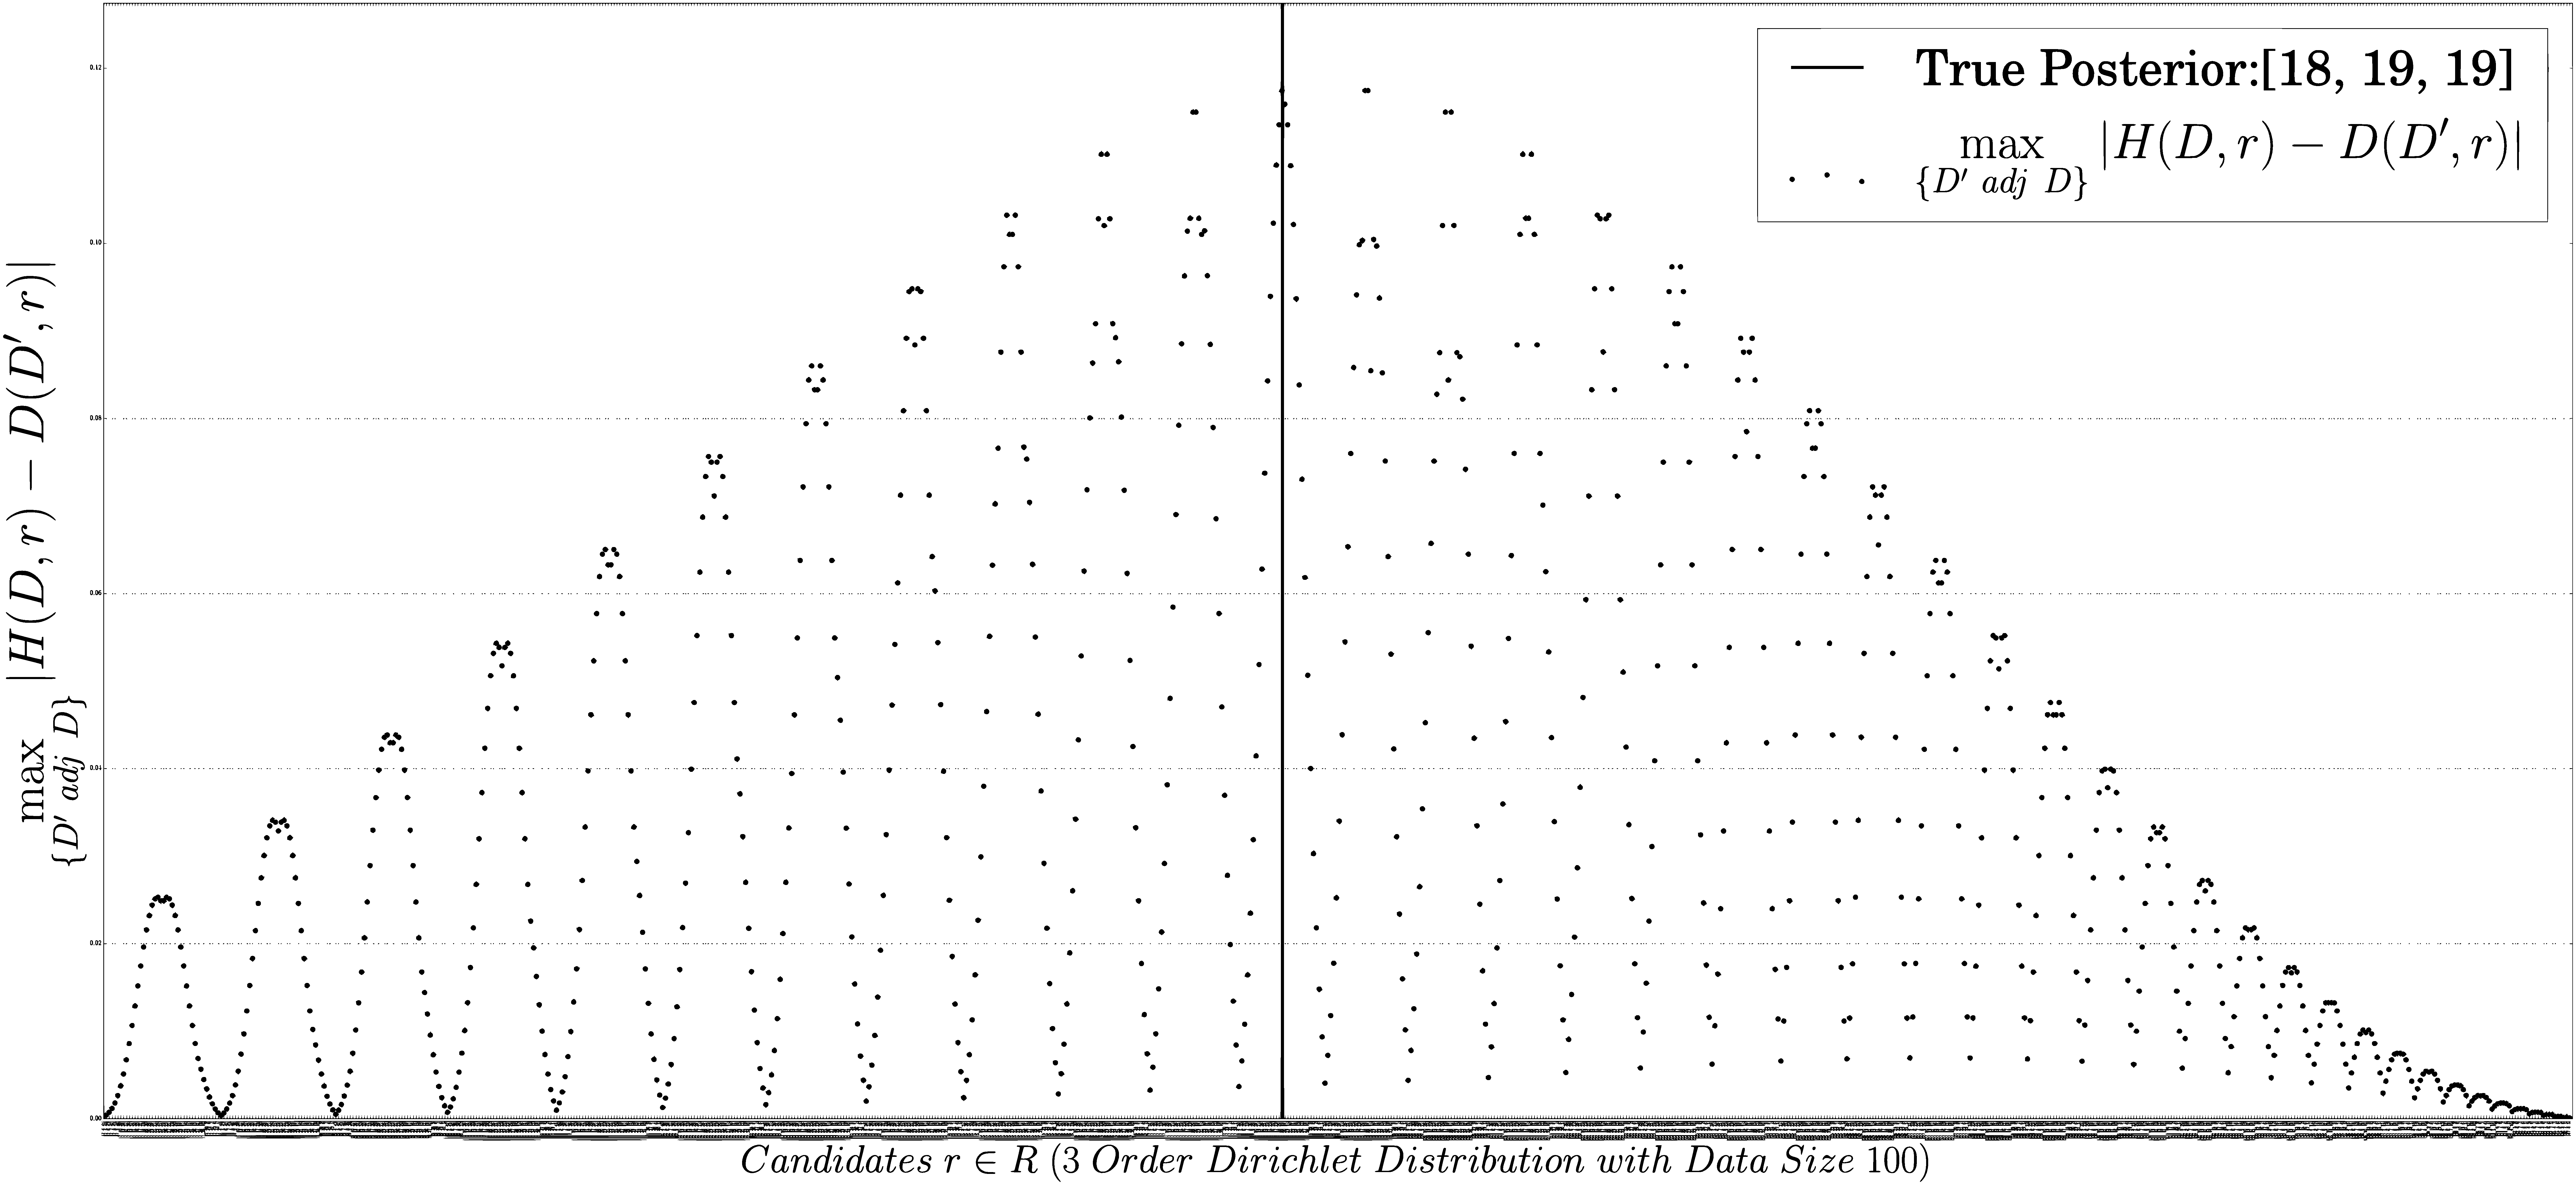
\includegraphics[width=1.0\textwidth]{efficiency}
\label{fig_efficiency}
\caption{Experimental Results for Finding the Local Sensitivity Efficiently}
\end{figure}

\subsection{Experimental Evaluations on Accuracy}
In this section, we do some experiments in order to study the accuracy property of these mechanisms, including the exponential mechanism with three kinds of sensitivity and the Laplace mechanism.

\subsubsection{Based on Hellinger Distance}
\label{subsec_accuracy_hellinger}
% \begin{figure*}
% \begin{center}
% \centering
%   \subfigure[Data size $n = 300$ with global $\epsilon = 0.5$]{
%     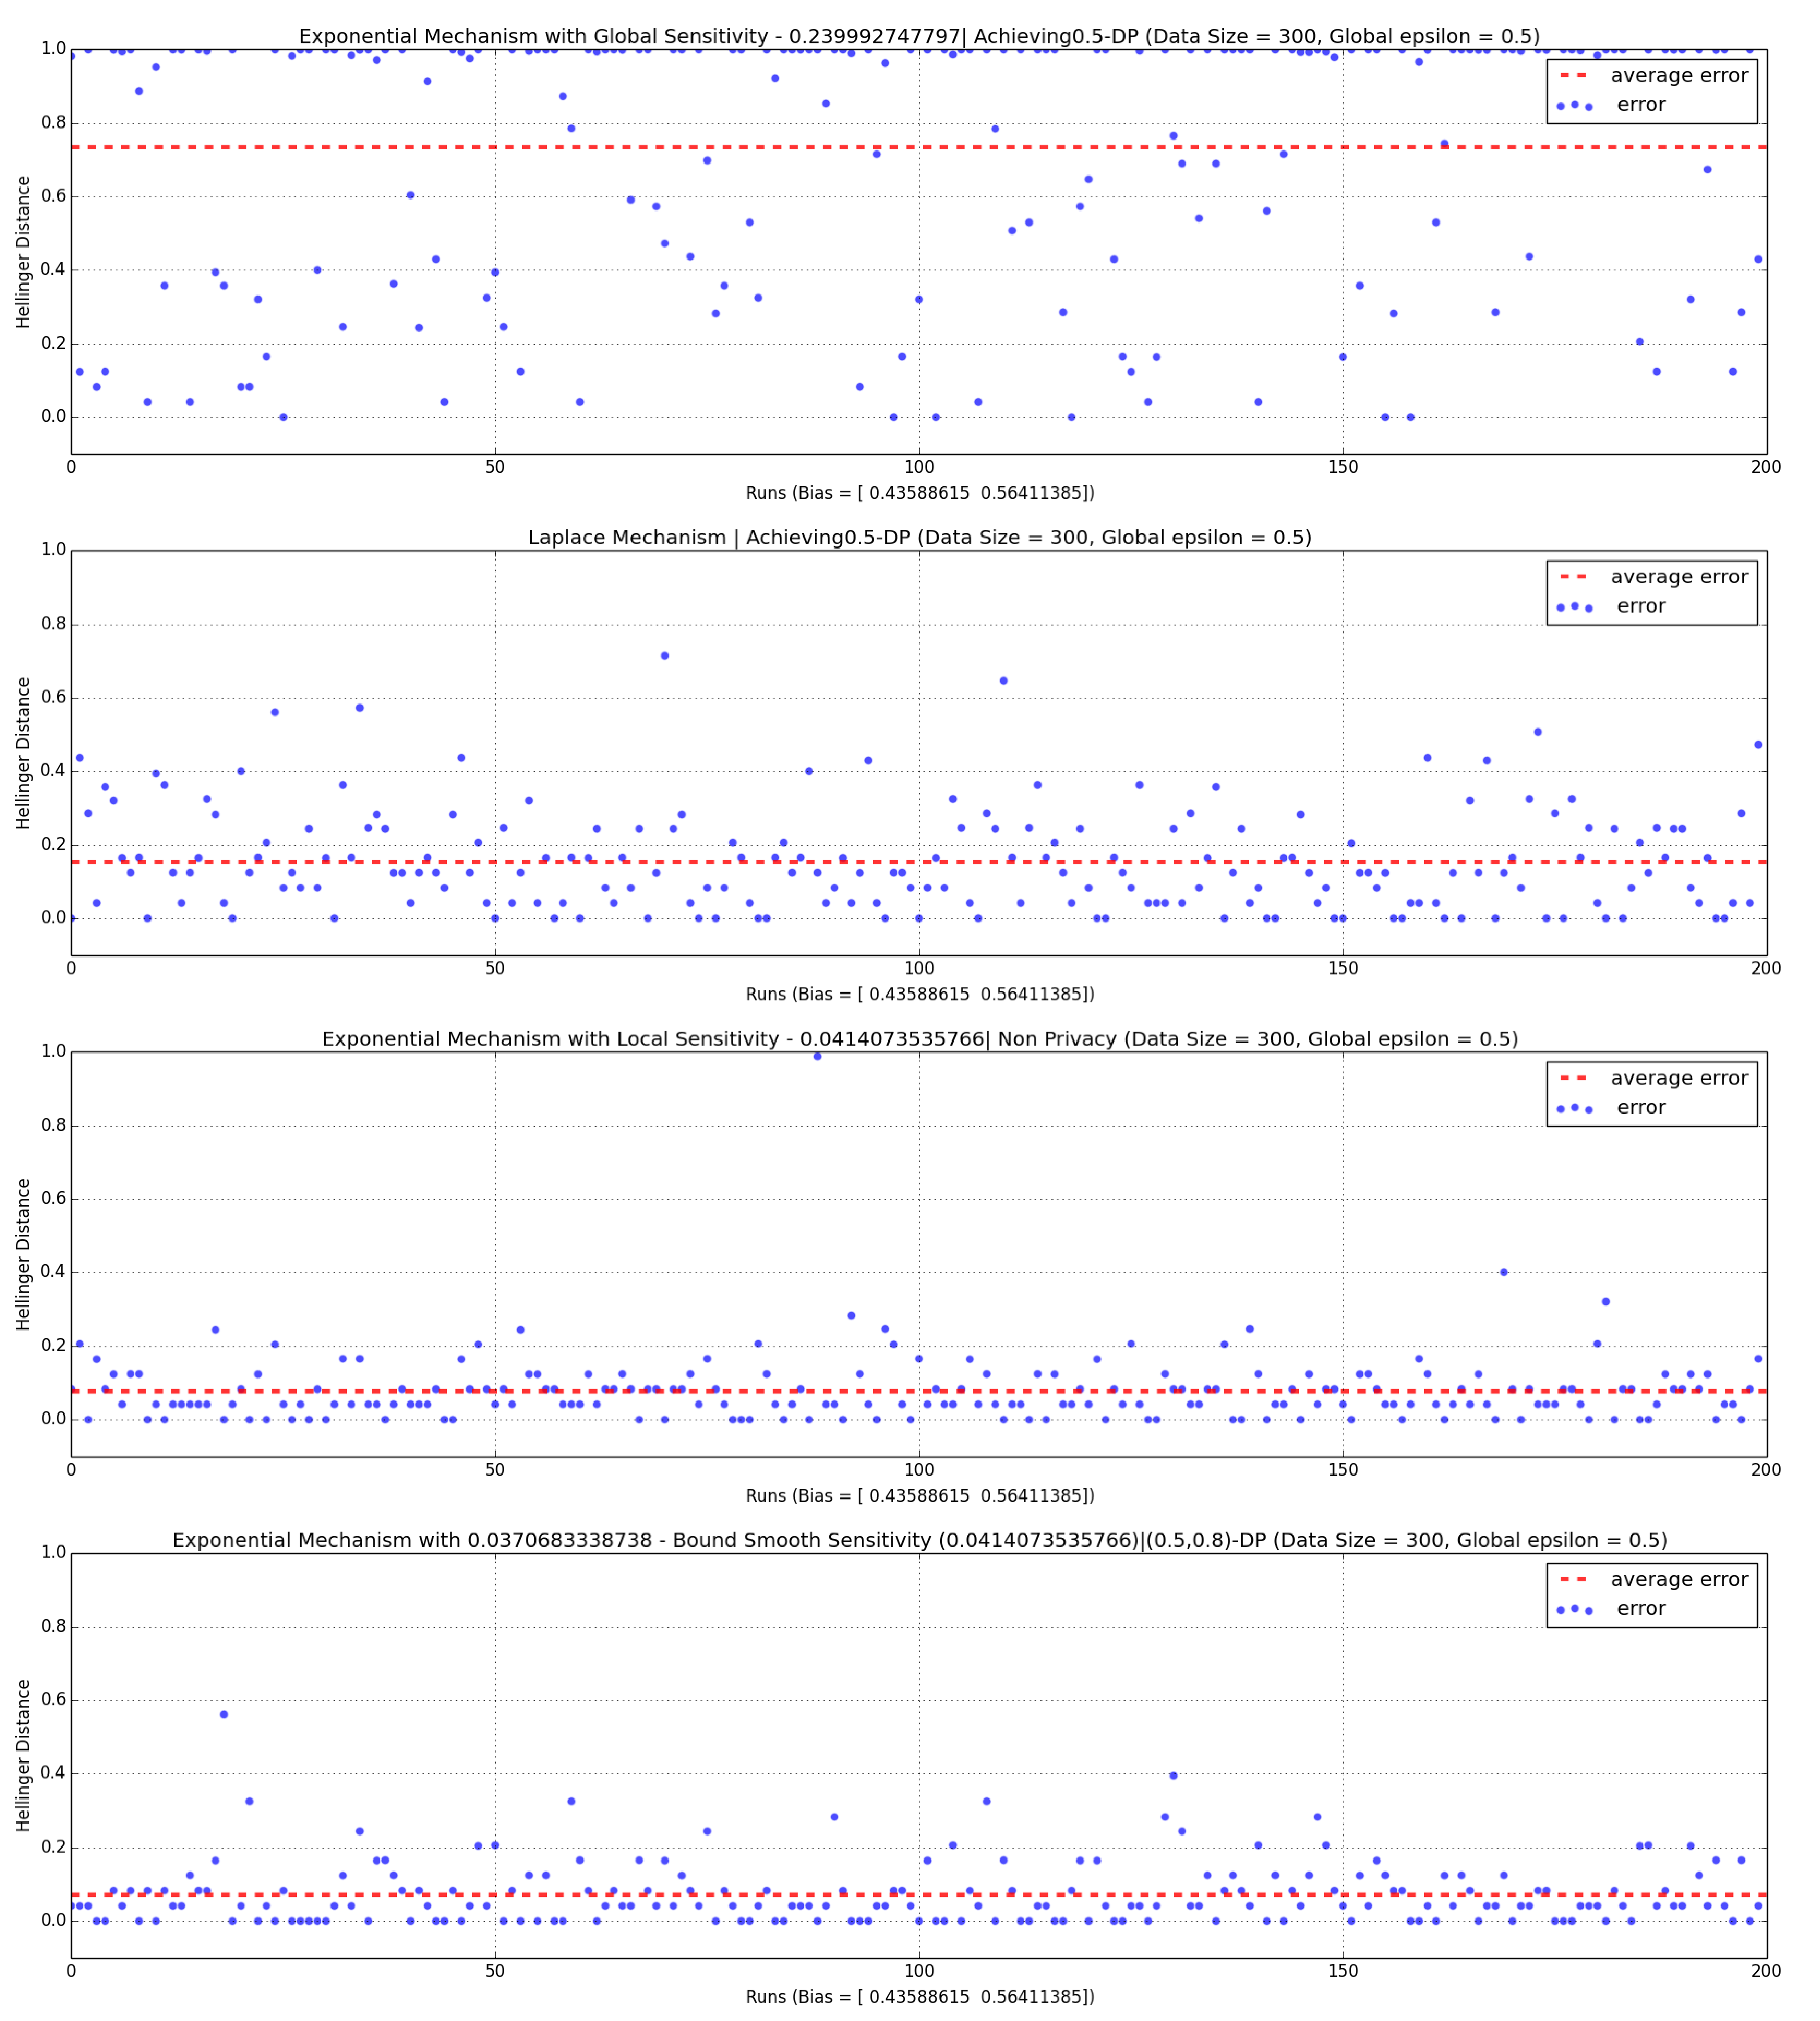
\includegraphics[width=0.48\textwidth]{accuracy_1.eps}}
%   \subfigure[Data size $n = 200$ with global $\epsilon = 0.8$]{
%     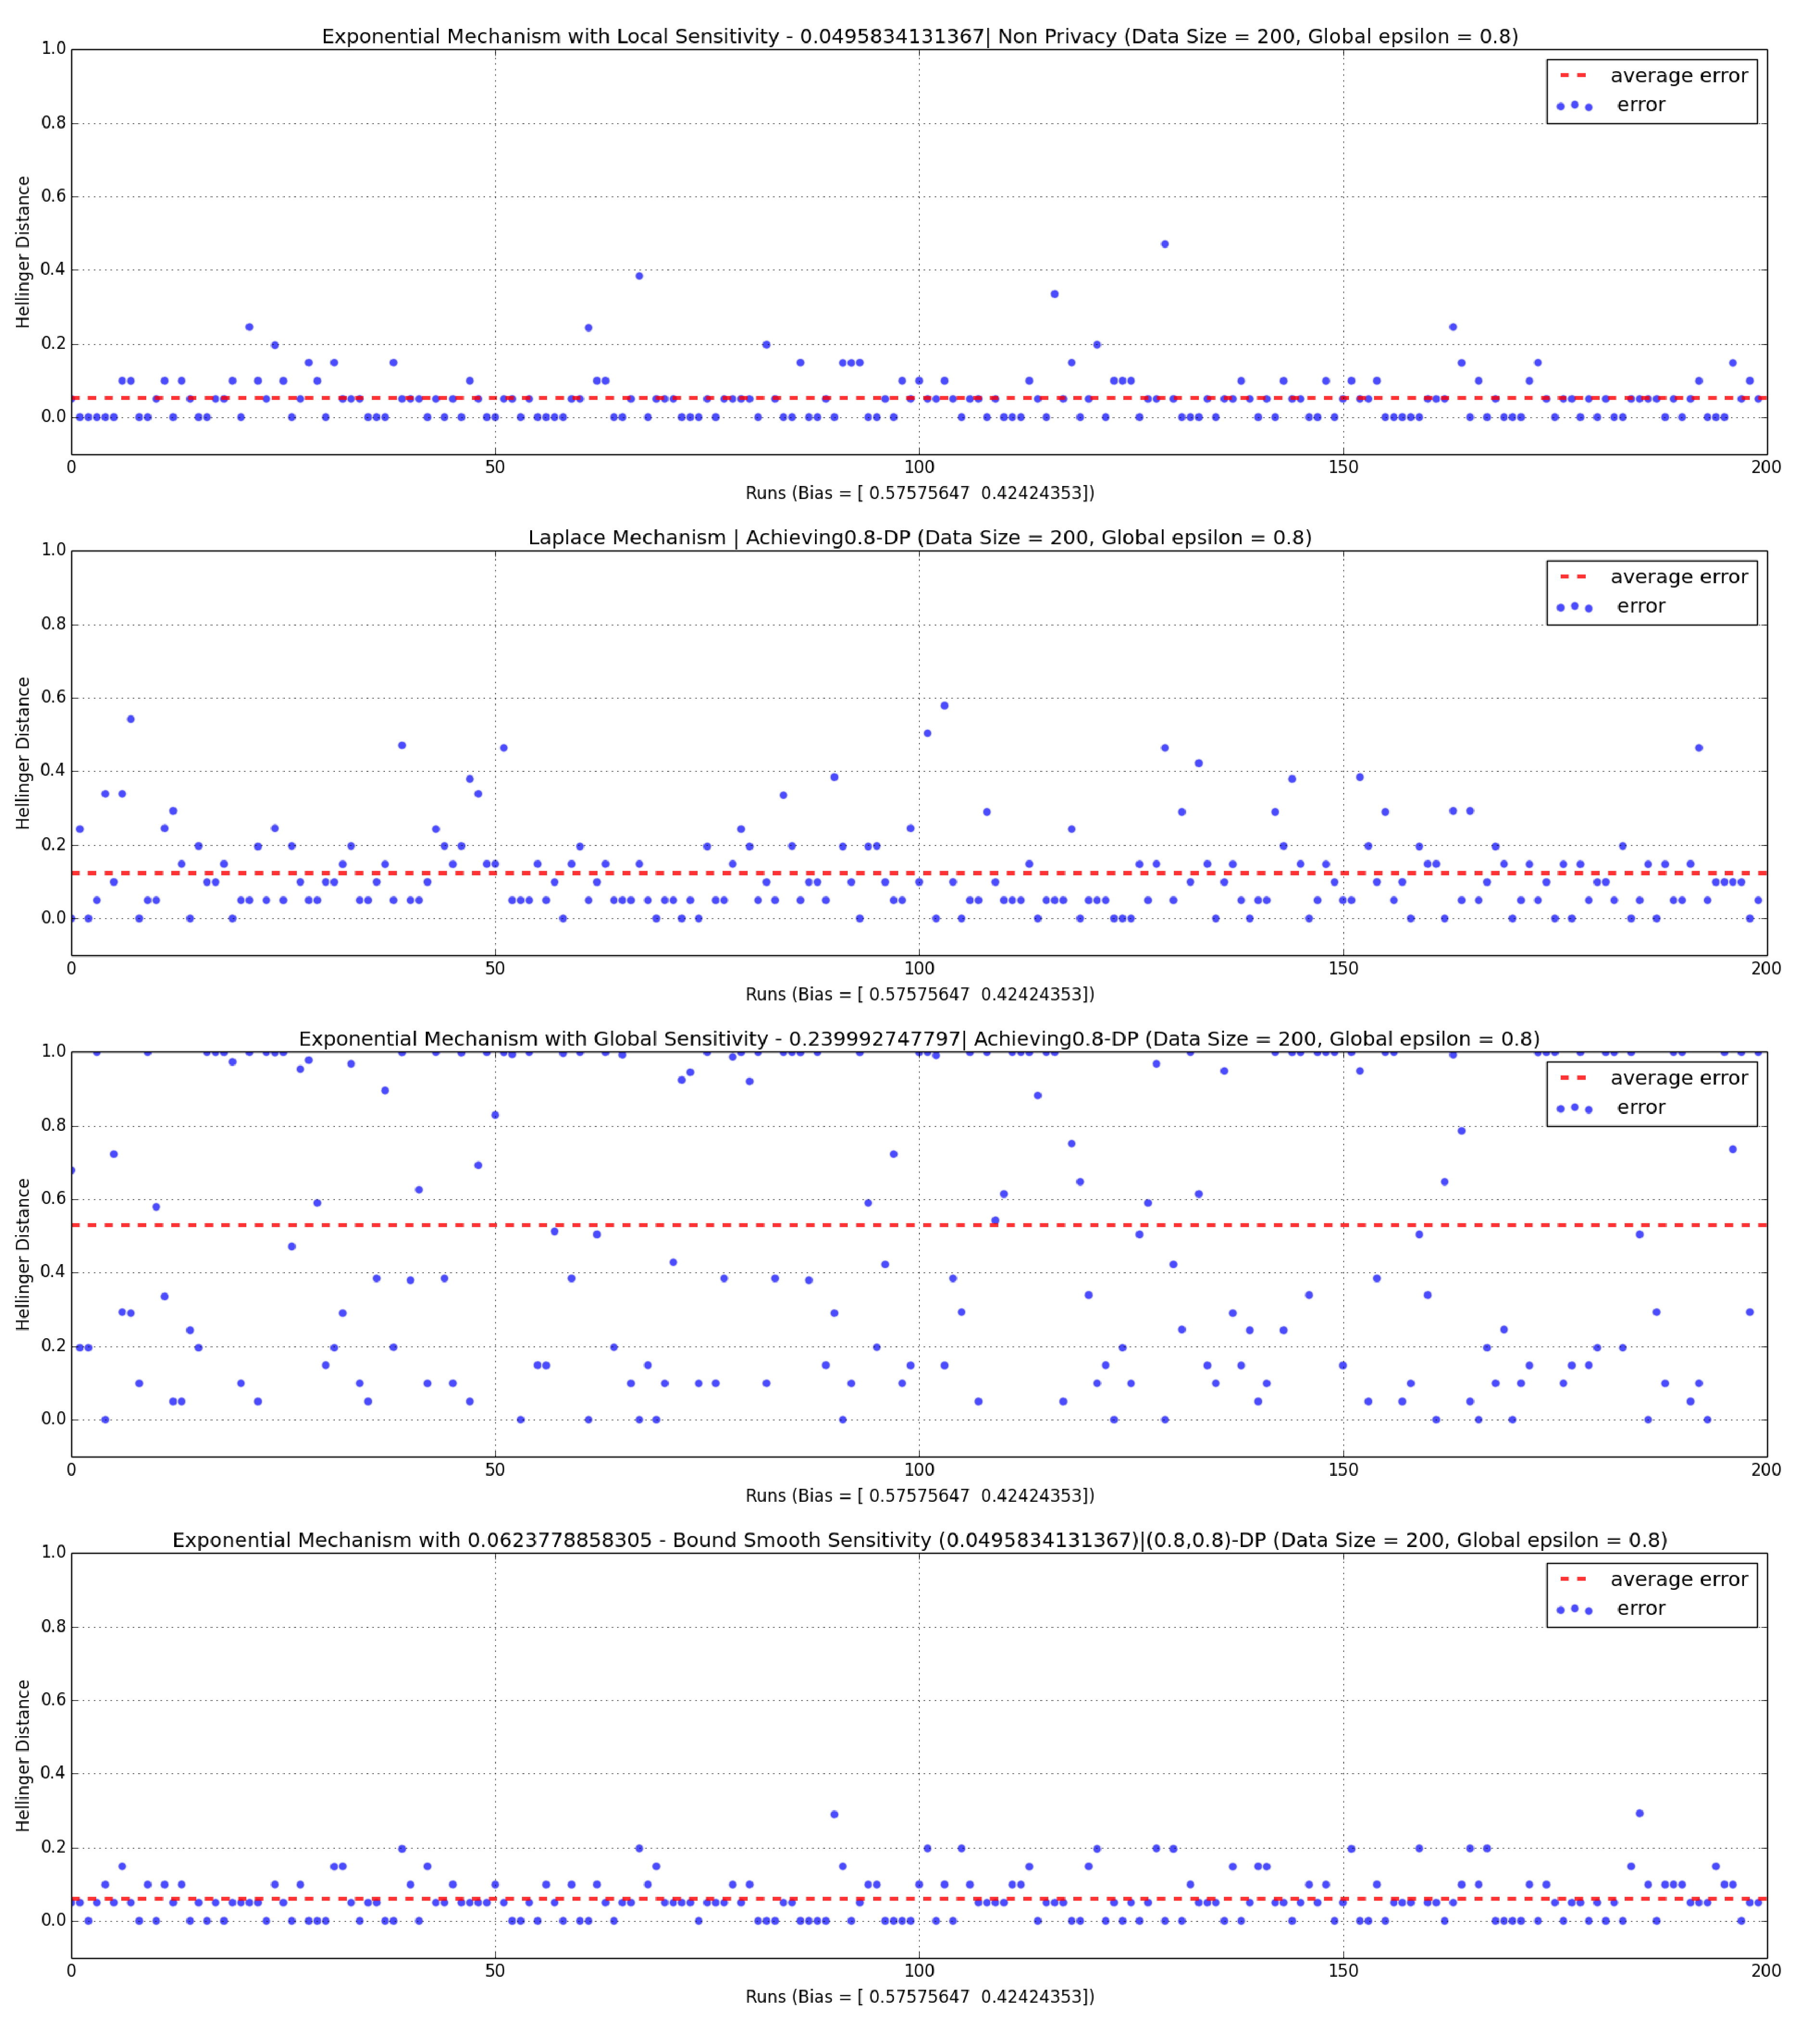
\includegraphics[width=0.48\textwidth]{accuracy_2.eps}} 
% \caption{The experimental results of accuracy of four algorithms}
% \label{fig_data}
% \end{center}
% \end{figure*}

\begin{figure*}
\begin{center}
\centering
  \subfigure[Data size $n = 500$ with global $\epsilon = 0.5$]{
    \includegraphics[width=0.48\textwidth]{accuracy_box_2.eps}}
  \subfigure[Data size $n = 300$ with global $\epsilon = 0.5$]{
    \includegraphics[width=0.48\textwidth]{accuracy_box_1.eps}} 
\caption{The experimental results of accuracy of algorithms with Beta prior distribution $\betad(7,4)$ based on Hellinger distance}
\label{fig_beta_hellinger}
\end{center}
\end{figure*}

\begin{figure*}
\begin{center}
\centering
  \subfigure[Data size $n = 100$, the exponential mechanism with global sensitivity 0.239992747797 is 0.8 -DP, with local sensitivity 0.08 is Non-Private and with 0.0699407108115 - bound smooth sensitivity 0.09 is (0.8,0.8)-DP]{
    \includegraphics[width=0.48\textwidth]{accuracy_dirichlet_hellinger_1.eps}}
  \subfigure[Data size $n = 120$, the exponential mechanism with global sensitivity 0.239992747797 is 0.8 -DP, with local sensitivity 0.0945 is Non-Private, with 0.0677791100173 - bound smooth sensitivity 0.096 is (0.8,0.8)-DP]{
    \includegraphics[width=0.48\textwidth]{accuracy_dirichlet_hellinger_2.eps}} 
\caption{The experimental results of accuracy of algorithms with Dirichlet prior distribution $\dirichlet(7, 4, 5)$ based on Hellinger distance}
\label{fig_dirichlet_hellinger}
\end{center}
\end{figure*}

We first analyzed the accuracy based on the Hellinger distance. By repeating the experiments for 10000 times and plotting the accuracy of each execution, we got two groups of results under different parameters setting as in Fig. \ref{fig_beta_hellinger} and Fig. \ref{fig_dirichlet_hellinger}. X-axis is labeled with different mechanisms. We took four mechanisms in our experiments: our newly designed exponential mechanism with smooth sensitivity named ``ExpoMech of SS'', exponential mechanism with local sensitivity named `` ExpoMech of LS'', exponential mechanism with global sensitivity named `` ExpoMech of GS'' and Laplace mechanism named ``LaplaceMech''. Y-axis is the accuracy measured by Hellinger distance between output $z$ of each execution and the correct inference result $\bysinfer(x)$, $\hlg(z, \bysinfer(x))$.

When prior distribution is $\betad$, under data size $n = 500$ and $300$, we obtained two plots in Fig. \ref{fig_beta_hellinger}. It is shown that our ExpoMech of SS is slightly better than Laplace mechanism and much more better than it with global sensitivity.

To have more experimental results, we then extended the $\betad$ to the Dirichlet distribution $\dirichlet$ as well as increased the data size, plotted in Fig. \ref{fig_dirichlet_hellinger}.

In both of the two cases, the performances of our exponential mechanism with smooth sensitivity and Laplace mechanism are very close. We can obtain some preliminary conclusions: 
\begin{enumerate}
	\item Our exponential mechanism with smooth sensitivity can have similar accuracy as it with local sensitivity. Both of the two exponential mechanisms are do much better than it with global sensitivity.
	\item The accuracy of our exponential mechanism is better than Laplace mechanism. But the advantages are not significant.
\end{enumerate} 

So we need to have a further exploration on the accuracy trade-off between Laplace mechanism and our exponential mechanism.

\subsubsection{Based on $L_1$ Norm}
\label{subsec_accuracy_l1}
In this section, we will study the accuracy of these four mechanisms based on $l_1$ norm, with the Dirichlet distribution $\dirichlet(7,4,5)$ and data size $150$ for comparison, as in Fig. \ref{fig_dirichlet_hellinger_l1}.

\begin{figure*}
\begin{center}
\centering
  \subfigure[accuracy measurement based on Hellinger distance]{
    \includegraphics[width=0.48\textwidth]{accuracy_compare_dirichlet_hellinger.eps}}
  \subfigure[accuracy measurement based on $l_1$ norm]{
    \includegraphics[width=0.48\textwidth]{accuracy_compare_dirichlet_l1.eps}} 
\caption{The experimental results of accuracy of algorithms with Dirichlet prior distribution $\dirichlet(7, 4, 5)$ based on Hellinger distance and $l_1$  norm, where data size $n = 150$, the exponential mechanism with global sensitivity 0.239992747797 is 0.8 -DP, with local sensitivity 0.0945 is Non-Private, with 0.0677791100173 - bound smooth sensitivity 0.096 is (0.8,0.8)-DP}
\label{fig_dirichlet_hellinger_l1}
\end{center}
\end{figure*}

The results based on $l_1$ norm are actually very similar to results based on Hellinegr distance.


\subsection{Evaluations on Accuracy Trade-off Between Laplace and Our Exponential Mechanism with Smooth Sensitivity}
\label{subsec_accuracy_tradeoff}
Based on accuracy study in Sec. \ref{subsec_accuracy_hellinger} and \ref{subsec_accuracy_l1}, we are going to have a further study on the accuracy relationship between Laplace mechanism and our exponential mechanism. We will do analysis both in theory and experiment and do some concrete case studies.

\subsubsection{Theory Analysis}
In this part, we will do theory analysis on the two mechanisms' discrete probabilities of outputting each candidate separately. In following analysis, we will count the probabilities wrt. the steps from correct answer, in order to be more concise and comparable to the experiment results from Sec. \ref{subsec_accuracy_hellinger}. For example, in the case where the correct posterior distribution is $\betad(5,5)$, the candidate $\betad(4,6)$ and $\betad(6,4)$ are of $1$ steps from $\betad(5,5)$; when correct posterior distribution is $\dirichlet(5,5,5)$, the candidate $\dirichlet(4,5,3)$, $\dirichlet(4,3,5)$, $\dirichlet(5,4,3)$, $\dirichlet(5,3,4)$, $\dirichlet(3,5,4)$ and $\dirichlet(5,5,5)$ are all of $1$ step from $\dirichlet(5,5,5)$. Under the Hellinger distance measurement, if candidates are of the same steps from correct answer, they also have the same Hellinger distance from correct answer. i.e for every $\hlg(\bysinfer(x), z) = c$, it will have a corresponding steps $step(\hlg(\bysinfer(x), z) = c) = k$. This will make the results more clear and observable.


\begin{itemize}

	\item In our exponential mechanism, the probability of outputting candidates wrt. steps (i.e., the hellinger distance) from the correct answer is calculated as:

	\begin{equation*}
	\underset{z \thicksim \hexpmech(x)}{Pr}[ \hlg(\bysinfer(x), z) = c] = \sum\limits_{\{z| \hlg(\bysinfer(x), z) = c\}}\frac{exp(\frac{- \epsilon c}{S(x)})}
	{\Sigma_{r' \in R}\ exp(\frac{-\epsilon \hlg(\bysinfer(x),r')}{2 S_\beta(x)})},
	\end{equation*}

	Each candidate will occupy a portion of ``$1$'' as their outputting probability. Supposing candidates within three steps from the correct answer are good answers, the portion occupied by the good answers is decreasing when the size of candidate set increasing. That's to say, the probabilities of outputting good answers are decreasing when the data size and dimension of prior distribution increasing. More specifically, the candidate set size is $\sim n^{m-1}$, which means the probabilities of outputting good answers are decreasing with speed $\sim n^{m-1}$.

	\item However in Laplace mechanism, the probability of producing noise has little relevance with the size of the candidate set. In $m$ dimensional Dirichlet distribution, when the correct posterior distribution is $\dirichlet(\alpha_1, \alpha_2, \cdots, \alpha_m)$, we are adding Laplace noise in this way: $\dirichlet(\alpha_1 + Lap_1, \alpha_2 + Lap_2, \cdots, n - (\alpha_1 + Lap_1 + \alpha_{m-1} + Lap_{m-1}))$ where $Lap_i \sim Floor(Lap(\frac{2}{\epsilon}))$ are i.i.d. So we will have a list of noise $L_{noise} = \{|Lap_1|, |Lap_2|,\cdots ,|Lap_{m-1}|\}$ by taking the absolute value of each noise $|Lap_i|$. In order to get the probability of a single candidate, we also need to have the set of noises $S_{noise}$ obtained from $L_{noise}$ by removing its duplicate values and the list $L_{noise/0}$ by removing 0s from $L_{noise}$. Then, the probabilities of outputting a single candidate in Laplace mechanism can be obtained by: 

	\begin{equation*}
	\begin{split}
	Pr[(Lap_1, Lap_2, \cdots, Lap_{m-1})]  
	& = \frac{1}{|S_{noise}|! \times 2^{|L_{noise/0}|}} \times Pr[(|Lap_1|, |Lap_2|, \cdots, |Lap_{m-1}|)] \\
	& = \frac{1}{|S_{noise}|! \times 2^{|L_{noise/0}|}} \times Pr[|Lap_1| \leq Lap(\frac{2}{\epsilon}) < |Lap_1| + 1] \\
	& \times Pr[|Lap_2| \leq Lap(\frac{2}{\epsilon}) < |Lap_2| + 1] \times \cdots \\
	& \times Pr[|Lap_{m-1}| \leq Lap(\frac{2}{\epsilon}) < |Lap_{m-1}| + 1]
	\end{split}
	\end{equation*}

	By summing up the probability value of candidates whose steps from correct answer are the same, we can finally get the probability wrt. steps from correct answer in Laplace mechanism.

	From analysis above, we can see the probabilities of outputting the good answers will not change a lot as the size of the candidate set increasing. Specifically, we can easily have two upper bounds: $|S_{noise}| \leq (m-1)$ and $|L_{noise/0}| \leq (m-1)$. From the two upper bounds, we can see that the probabilities of outputting good answers are decreasing with speed upper bounded by $(m-1)! \times 2^{m-1}$. Since $n \gg 2$ and $m$ is usually smaller than $10$, it is easy to see that the decay speed $(m-1)! \times 2^{m-1}$ in Laplace mechanism is much more smaller than $n^{m-1}$ in our exponential mechanism. Moreover, when the steps are small, $0$ for example, $|S_{noise}| = |L_{noise/0}|  = 0$, which means the probability of correct answer will decrease very little no matter how large the candidate set is. 

	\item Then, we do some concrete cases analysis.

	\begin{itemize}

		\item when the prior is $\betad(1,1)$, the observed data set $x = (1,1,0,0,1,1,0,0)$, it is easy to compute the posterior distribution: $\betad(5,5)$, the probability from the two mechanisms are: 

		\begin{center}
		 \begin{tabular}{c | c | c} 
		 \hline
		 Hellinger Distance / steps & Our Exponential Mechanism & Laplace Mechanism  \\
		 \hline\hline
		 $Pr[\hlg(\bysinfer(x), r) = 0.83737258593] / 4		$ & 0.0431193490585 & 0.066561234758\\ 
		 \hline
		 $Pr[\hlg(\bysinfer(x), r) = 0.662174391701 ] / 3	$ & 0.0785621424847 & 0.0992976939175  \\
		 \hline
		 $Pr[\hlg(\bysinfer(x), r) = 0.457635865026 ] / 2	$ & 0.158265808563 & 0.148134752205  \\
		 \hline
		 $Pr[\hlg(\bysinfer(x), r) = 0.233629480709 ] / 1	$ & 0.340809715054 & 0.220991081918  \\
		 \hline
		 $Pr[\hlg(\bysinfer(x), r) = 0.0 ] / 0 				$ & 0.37924298484 & 0.329679953964 \\
		 \hline
		\end{tabular}
		\end{center}

		Here, there are only 5 kinds of steps from correct answer. Our mechanism in the second column is clearly better than Laplace mechanism in the third column. When the candidates are close to correct answer (for example, $0, 1, 2$ steps from correct answer), our mechanism can output them with higher probabilities than Laplace mechanism. On the other hand, when candidates are far away from correct answer (for example, $3, 4$ steps), our mechanism can output them with lower probabilities.

		\item when the prior is $\dirichlet(1,1,1)$, the observed data set $x = (20,20,20)$ (suppose a black box will produce $A$, $B$, $C$ with a certain distribution, after observing this black box continuously for 60 times, we get $20$ times $A$, $20$ times $B$ and $20$ times $C$), we can get the posterior distribution $\dirichlet(21,21,21)$

		\begin{center}
		 \begin{tabular}{c | c | c} 
		 \hline
		 Hellinger Distance / steps & Our Exponential Mechanism & Laplace Mechanism  \\
		 \hline\hline
		 $Pr[\hlg(\bysinfer(x), r) = 0.999999984481] / \cdots 	$ & 0.000149705644585 & 3.05988187701e-09\\ 
		 \hline
		 \multicolumn{3}{c}{$\cdots$}  \\
		 \hline
		 $Pr[\hlg(\bysinfer(x), r) = 0.187421762881] / 2		$ & 0.0548161224677 & 0.0285774941516 \\
		 \hline
		 $Pr[\hlg(\bysinfer(x), r) = 0.110122822057 ] / 1		$ & 0.192227323562 & 0.170131188571  \\
		 \hline
		 $Pr[\hlg(\bysinfer(x), r) = 0.0 ] / 0 					$ & 0.0713016293602 & 0.108688872046 \\
		 \hline
		\end{tabular}
		\end{center}

		In this case, it is hard to tell which one is better because Laplace mechanism can output some good answers (for example, the correct answer) better than our mechanism but cannot go better with other good answers.

		\item when the prior is $\dirichlet(1,1,1,1)$, the observed data set is $(1,1,1,50)$ (the same meaning as above), we can get the posterior distribution $\dirichlet(2,2,2,51)$. Some probabilities from the two mechanisms are listed as follows:
		\begin{center}
		 \begin{tabular}{c | c | c} 
		 \hline
		 Hellinger Distance / steps & Our Exponential Mechanism & Laplace Mechanism  \\
		 \hline\hline
		 $Pr[\hlg(\bysinfer(x), r) = 0.999999999998] / \cdots 	$ & 0.000213865923868 & 6.16388940464e-11\\ 
		 \hline
		 \multicolumn{3}{c}{$\cdots$}  \\
		 \hline
		 $Pr[\hlg(\bysinfer(x), r) = 0.340503311163] / 2		$ & 0.000388935212208 & 0.0360289071389 \\
		 \hline
		 $Pr[\hlg(\bysinfer(x), r) = 0.249722620018 ] / 1		$ & 0.000464587461035 & 0.0360289071389  \\
		 \hline
		 $Pr[\hlg(\bysinfer(x), r) = 0.0 ] / 0 					$ & 0.000252512987228 & 0.0358325423325 \\
		 \hline
		\end{tabular}
		\end{center}

		This case shows that the Laplace mechanism do much better than our exponential mechanism significantly. These good answers with few steps from correct answer can be outputted with higher probabilities in Laplace mechanism than in our mechanism. Moreover, in our mechanism the bad answers and good answers have very similar outputting probabilities.

	\end{itemize}  

\end{itemize}


\subsubsection{Experiment Analysis}
In this part, we will do some experiment analysis to study the accuracy trade-off between our exponential mechanism and Laplace mechanism. By computing the two mechanisms' discrete probabilities wrt. steps (i.e., Hellinegr distance) from correct answer under different settings, we got groups of results as in Fig. \ref{fig_theory_50_50}, \ref{fig_theory_20_20_20}, \ref{fig_theory_20_20_20_20} and \ref{fig_theory_1_1_1_77}. 

Subfigs (a) based on Sec. \ref{subsec_accuracy_hellinger} shows the average accuracy of these mechanisms by executing them for 10000 times. The x-axis is labeled with mechanisms and y-axis is the accuracy of every execution outputs measured by Hellinegr distance. Subfigs (b) are concrete probabilities of Laplace and our exponential mechanisms' wrt. the steps. The x-axis is the Hellinger distance from correct answer, i.e. steps from correct answer. Since they have the same meaning, we just use the Hellinger distance to label the x-axis here. The y-axis is the probability of output candidates with corresponding steps (i.e. Hellinger distance) from correct answer.


\begin{figure*}
\begin{center}
\centering
  \subfigure[accuracy measurement based on Hellinger distance]{
    \includegraphics[width=0.48\textwidth]{theory_compare_50_50.eps}}
  \subfigure[discrete probabilities wrt. hellinger distance]{
    \includegraphics[width=0.48\textwidth]{50_50.eps}} 
\caption{Settings: Dirichlet prior distribution $\dirichlet(1,1)$, observed data $x = (49, 49) $, $\epsilon = 0.8$ and $\delta = 0.000005$}
\label{fig_theory_50_50}
\end{center}
\end{figure*}


When the data size and the dimension of the prior distribution is small, our exponential mechanism can do better than Laplace, both in experiments and in theory, as shown in Fig. \ref{fig_theory_50_50}. In Subfig. \ref{fig_theory_50_50}(a), the experiment results show that the average Hellinger distance of our mechanism's outputs are smaller than Laplace mechanism, i.e., the average accuracy of our mechanism is higher than Laplace mechanism. In the mean time, the theory calculation results in Subfig. \ref{fig_theory_50_50}(b) also show that our exponential mechanism can output good answers with higher probabilities and output bad answers with lower probabilities than Laplace mechanism.


\begin{figure*}
\begin{center}
\centering
  \subfigure[accuracy measurement based on Hellinger distance]{
    \includegraphics[width=0.48\textwidth]{theory_compare_20_20_20.eps}}
  \subfigure[discrete probabilities wrt. hellinger distance]{
    \includegraphics[width=0.48\textwidth]{20_20_20.eps}} 
\caption{Settings: Dirichlet prior distribution $\dirichlet(1,1,1)$, observed data $x = (20,20,20)$, $\epsilon = 0.8$ and $\delta = 0.000005$}
\label{fig_theory_20_20_20}
\end{center}
\end{figure*}


In Fig. \ref{fig_theory_20_20_20}, we plotted the results under the case ($x = (20,20,20)$). SubFig. \ref{fig_theory_20_20_20}(a) shows that the average accuracy of Laplace mechanism is slightly better than our mechanism. Meanwhile, the SubFig. \ref{fig_theory_20_20_20}(b) shows the Laplace mechanism have higher probabilities on some good answers but lower on some other good answers. The advantage is not significant. So, we increase the data size and the dimension in next case to have a further study.


\begin{figure*}
\begin{center}
\centering
  \subfigure[accuracy measurement based on Hellinger distance]{
    \includegraphics[width=0.48\textwidth]{theory_compare_20_20_20_20.eps}}
  \subfigure[discrete probabilities wrt. hellinger distance]{
    \includegraphics[width=0.48\textwidth]{20_20_20_20.eps}} 
\caption{Settings: Dirichlet prior distribution $\dirichlet(1,1,1,1)$, observed data $x = (20,20,20,20) $, $\epsilon = 0.8$ and $\delta = 0.000005$}
\label{fig_theory_20_20_20_20}
\end{center}
\end{figure*}


Here we studied the case when data size $n = 80$ and observed data set $x=(20,20,20,20)$ and plotted these discrete probabilities, shown in Fig. \ref{fig_theory_20_20_20_20}.  Subfig. \ref{fig_theory_20_20_20_20}(a) shows that the Laplace mechanism is better than our exponential mechanism very obviously. Subfig \ref{fig_theory_20_20_20_20}(b) shows that the Laplace can output most of the good answers with higher probabilities than our exponential mechanism. The advantage in the SubFig. \ref{fig_theory_20_20_20_20}(a) is obvious but still not significant in SubFig. \ref{fig_theory_20_20_20_20}(b). So, we change the variance of the observed data set in the next case.


\begin{figure*}
\begin{center}
\centering
  \subfigure[accuracy measurement based on Hellinger distance]{
    \includegraphics[width=0.48\textwidth]{theory_compare_1_1_1_77.eps}}
  \subfigure[discrete probabilities wrt. hellinger distance]{
    \includegraphics[width=0.48\textwidth]{1_1_1_77.eps}} 
\caption{Settings: Dirichlet prior distribution $\dirichlet(1,1,1,1)$, observed data $x = (1,1,1,77) $, $\epsilon = 0.8$ and $\delta = 0.000005$}
\label{fig_theory_1_1_1_77}
\end{center}
\end{figure*}


In Fig. \ref{fig_theory_1_1_1_77}, we considered an edge case where the variance of the observed data set is small: $x=(1,1,1,77)$ and plotted these discrete probabilities. This plot can show clearly that the Laplace mechanism is much better than our exponential mechanism, both in (a) and (b). In Subfig. \ref{fig_theory_1_1_1_77}(b), the average accuracy of Laplace mechanism is conspicuously better than the other three exponential mechanisms. Also, in Subfig. \ref{fig_theory_1_1_1_77}(b), the Laplace mechanism can output good answers with much higher probabilities, even though their performances on bad answers are not so obviously. Moreover, no matter good answers or bad answers, their outputting probabilities are very close in our exponential mechanism. 

From the theory and experimental analysis above, we obtained some conclusions
\begin{enumerate}
	\item when the data size and the dimensions of the prior distribution are small (candidate set size $n^{m-1}$ around 5000, our exponential mechanism with smooth sensitivity can do better than Laplace mechanism. 

	\item when the observed data set is close to center (i.e., the variance is large), the performance of the two mechanisms are close to each other.

	\item The Laplace mechanism will beat us when the data size and the dimensions of the prior distribution increasing and when the variance of the observed data set is small.
\end{enumerate}


\subsection{Accuracy Evaluation wrt. Different Variables}
\label{subsubsec_vs_variables}

In this section, we evaluate the accuracy wrt. four variables, including data size, dimension, data variance and prior distribution, and some combinations of these variables. We experiment 1000 times under each value of variables and produce 4-quantile plots for each variable. In following 4-quantile plots, the y-axis is accuracy measured by Hellinger distance, x-axis is different value of variables. The blue boxes in plots represent our exponential mechanism and the next yellow box represents the Laplace mechanism under the same setting.

\subsubsection{Accuracy Evaluation wrt. Datasize}
\label{subsubsec_vs_datasize}

\begin{figure*}
\begin{center}
\centering
  \subfigure[two dimensions with $\betad (1,1)$ prior distribution]{
    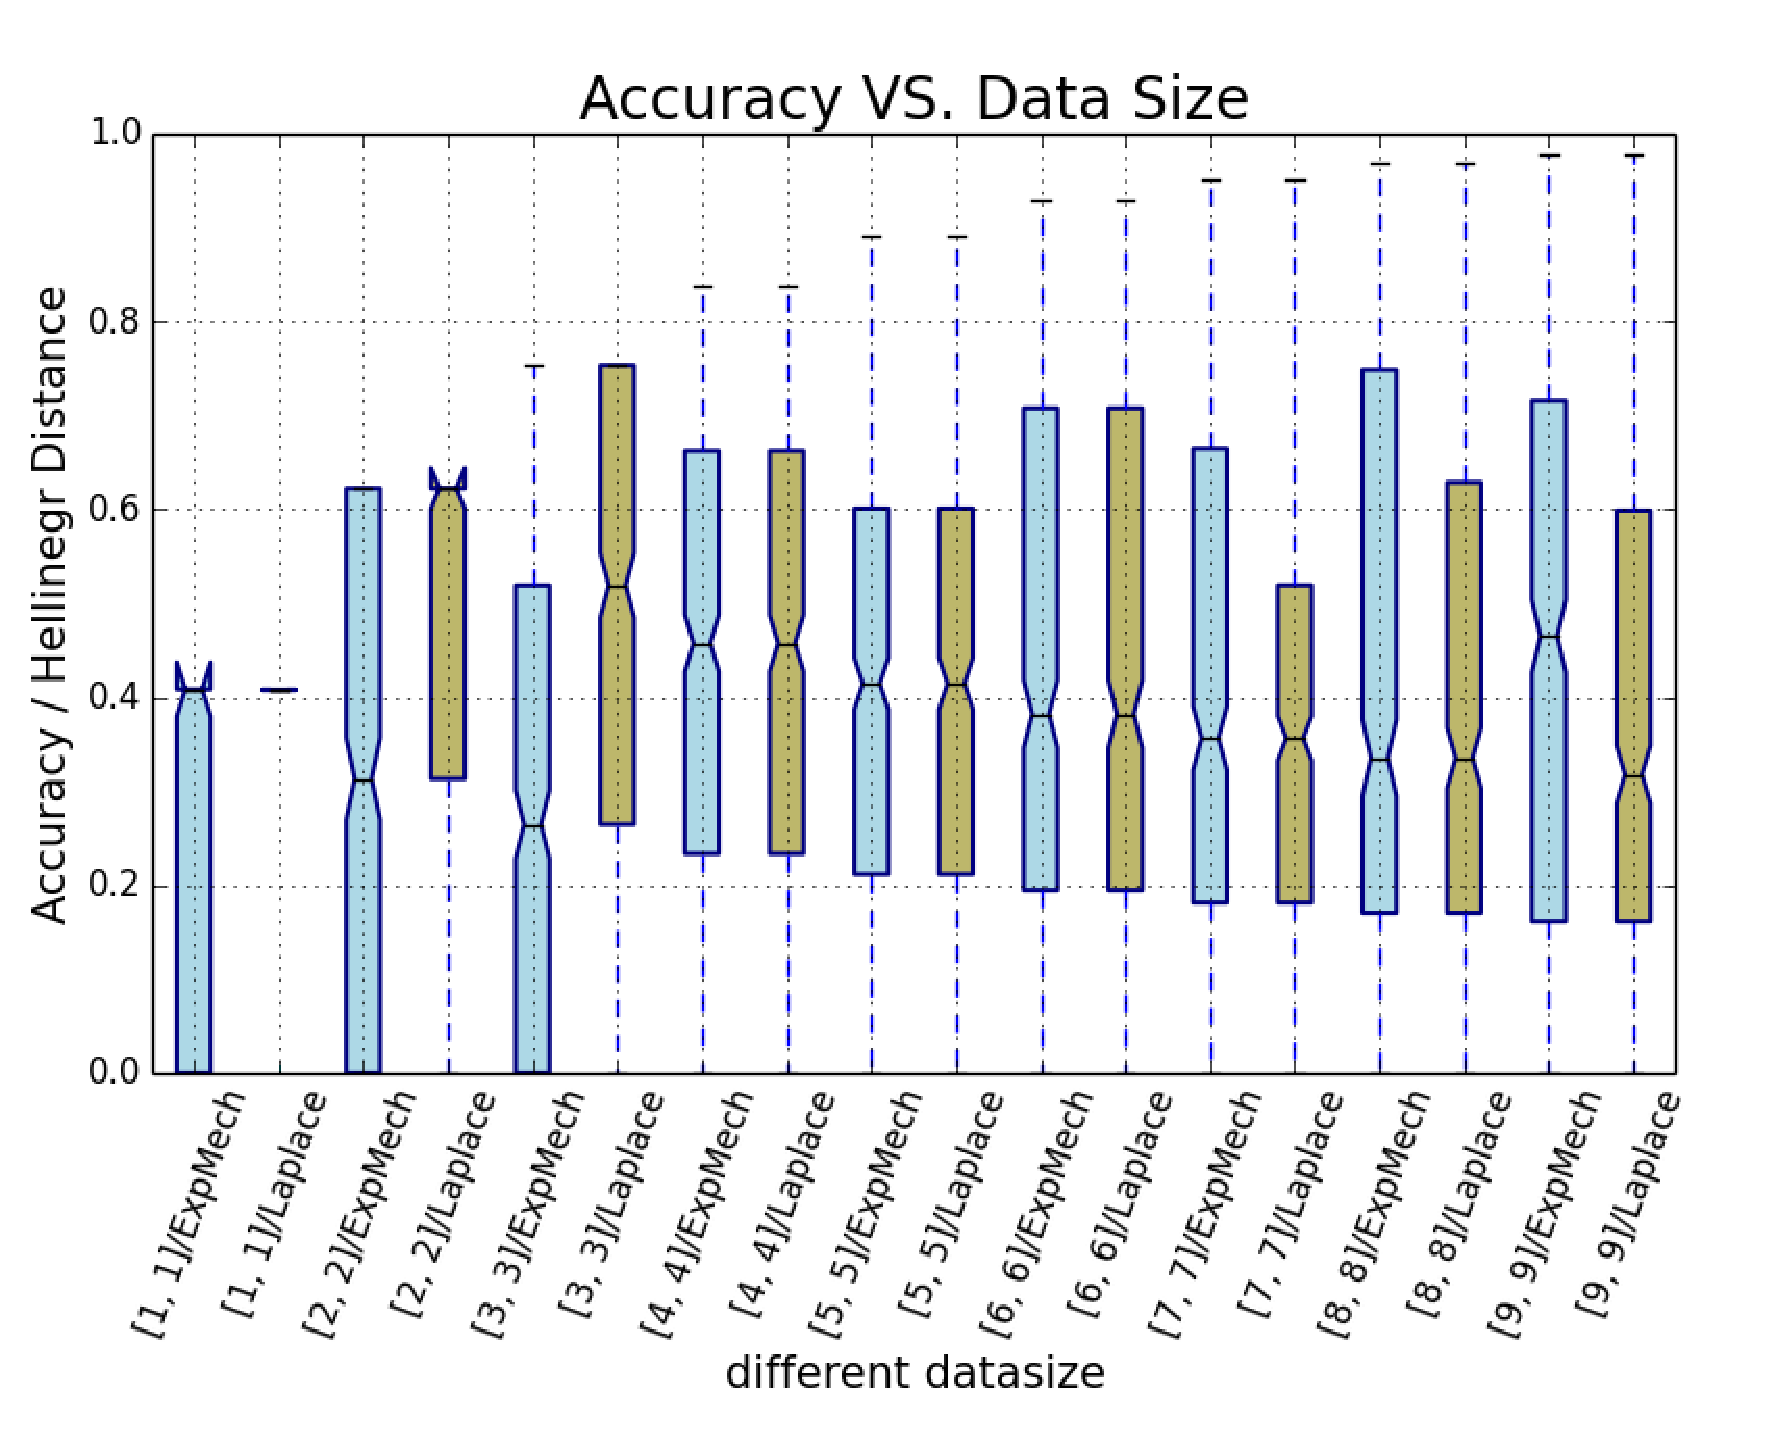
\includegraphics[width=0.48\textwidth]{accuracy_vs_datasize_1_1.eps}}
  \subfigure[three dimensions with $\dirichlet (1,1,1)$ prior distribution]{
    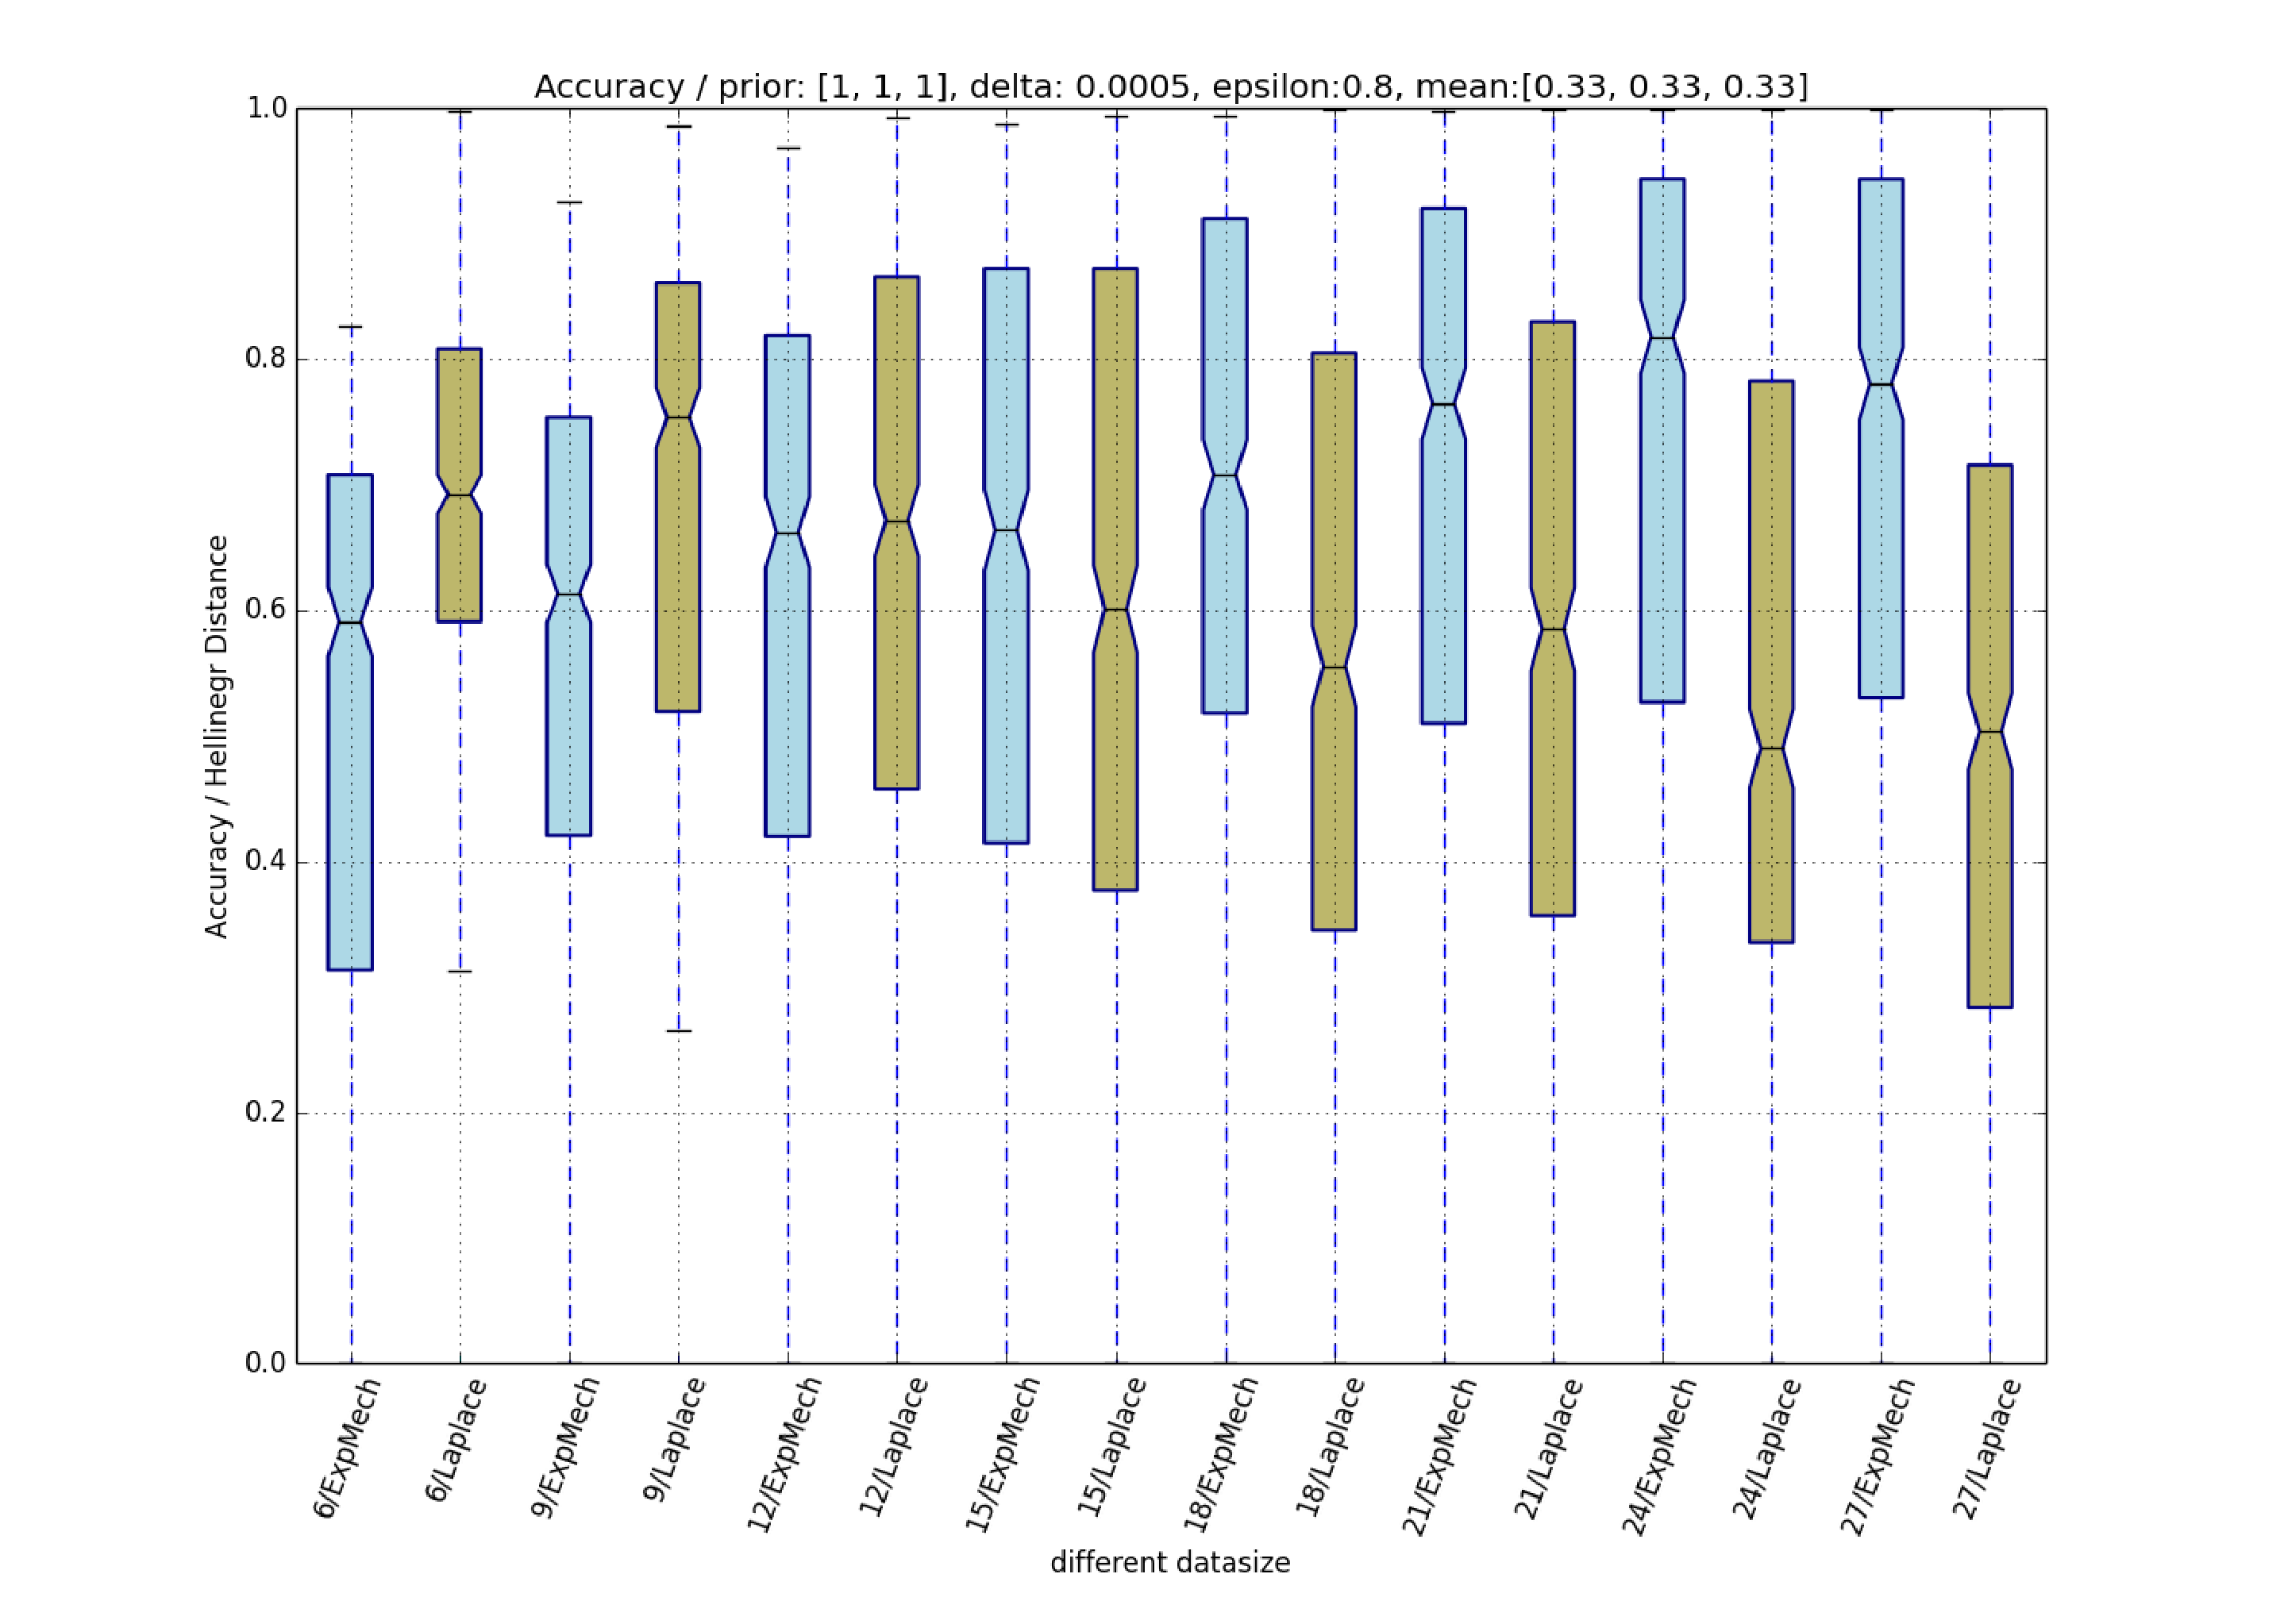
\includegraphics[width=0.48\textwidth]{accuracy_vs_datasize_1_1_1.eps}} 
\caption{Accuracy measurement based on Hellinger distance wrt. different datasizes. Settings: observed data are uniformly distributed, $\epsilon = 0.8$ and $\delta = 0.0005$}
\label{fig_vs_datasize}
\end{center}
\end{figure*}

In Fig. \ref{fig_vs_datasize}, both of the two plots show that when data size go larger, accuracy of our exponential mechanism are decreasing. In Fig. \ref{fig_vs_datasize}(a), when the data size is smaller than 12, we can beta Laplace mechanism but fail when data size larger than or equal to 12. Same as in Fig. \ref{fig_vs_datasize}(b), we can beat Laplace mechanism when data size is smaller than 15 and fail otherwise.

\subsubsection{Accuracy Evaluation wrt. Dimensions}
\label{subsubsec_vs_dimension}


\begin{figure}[h]
\centering
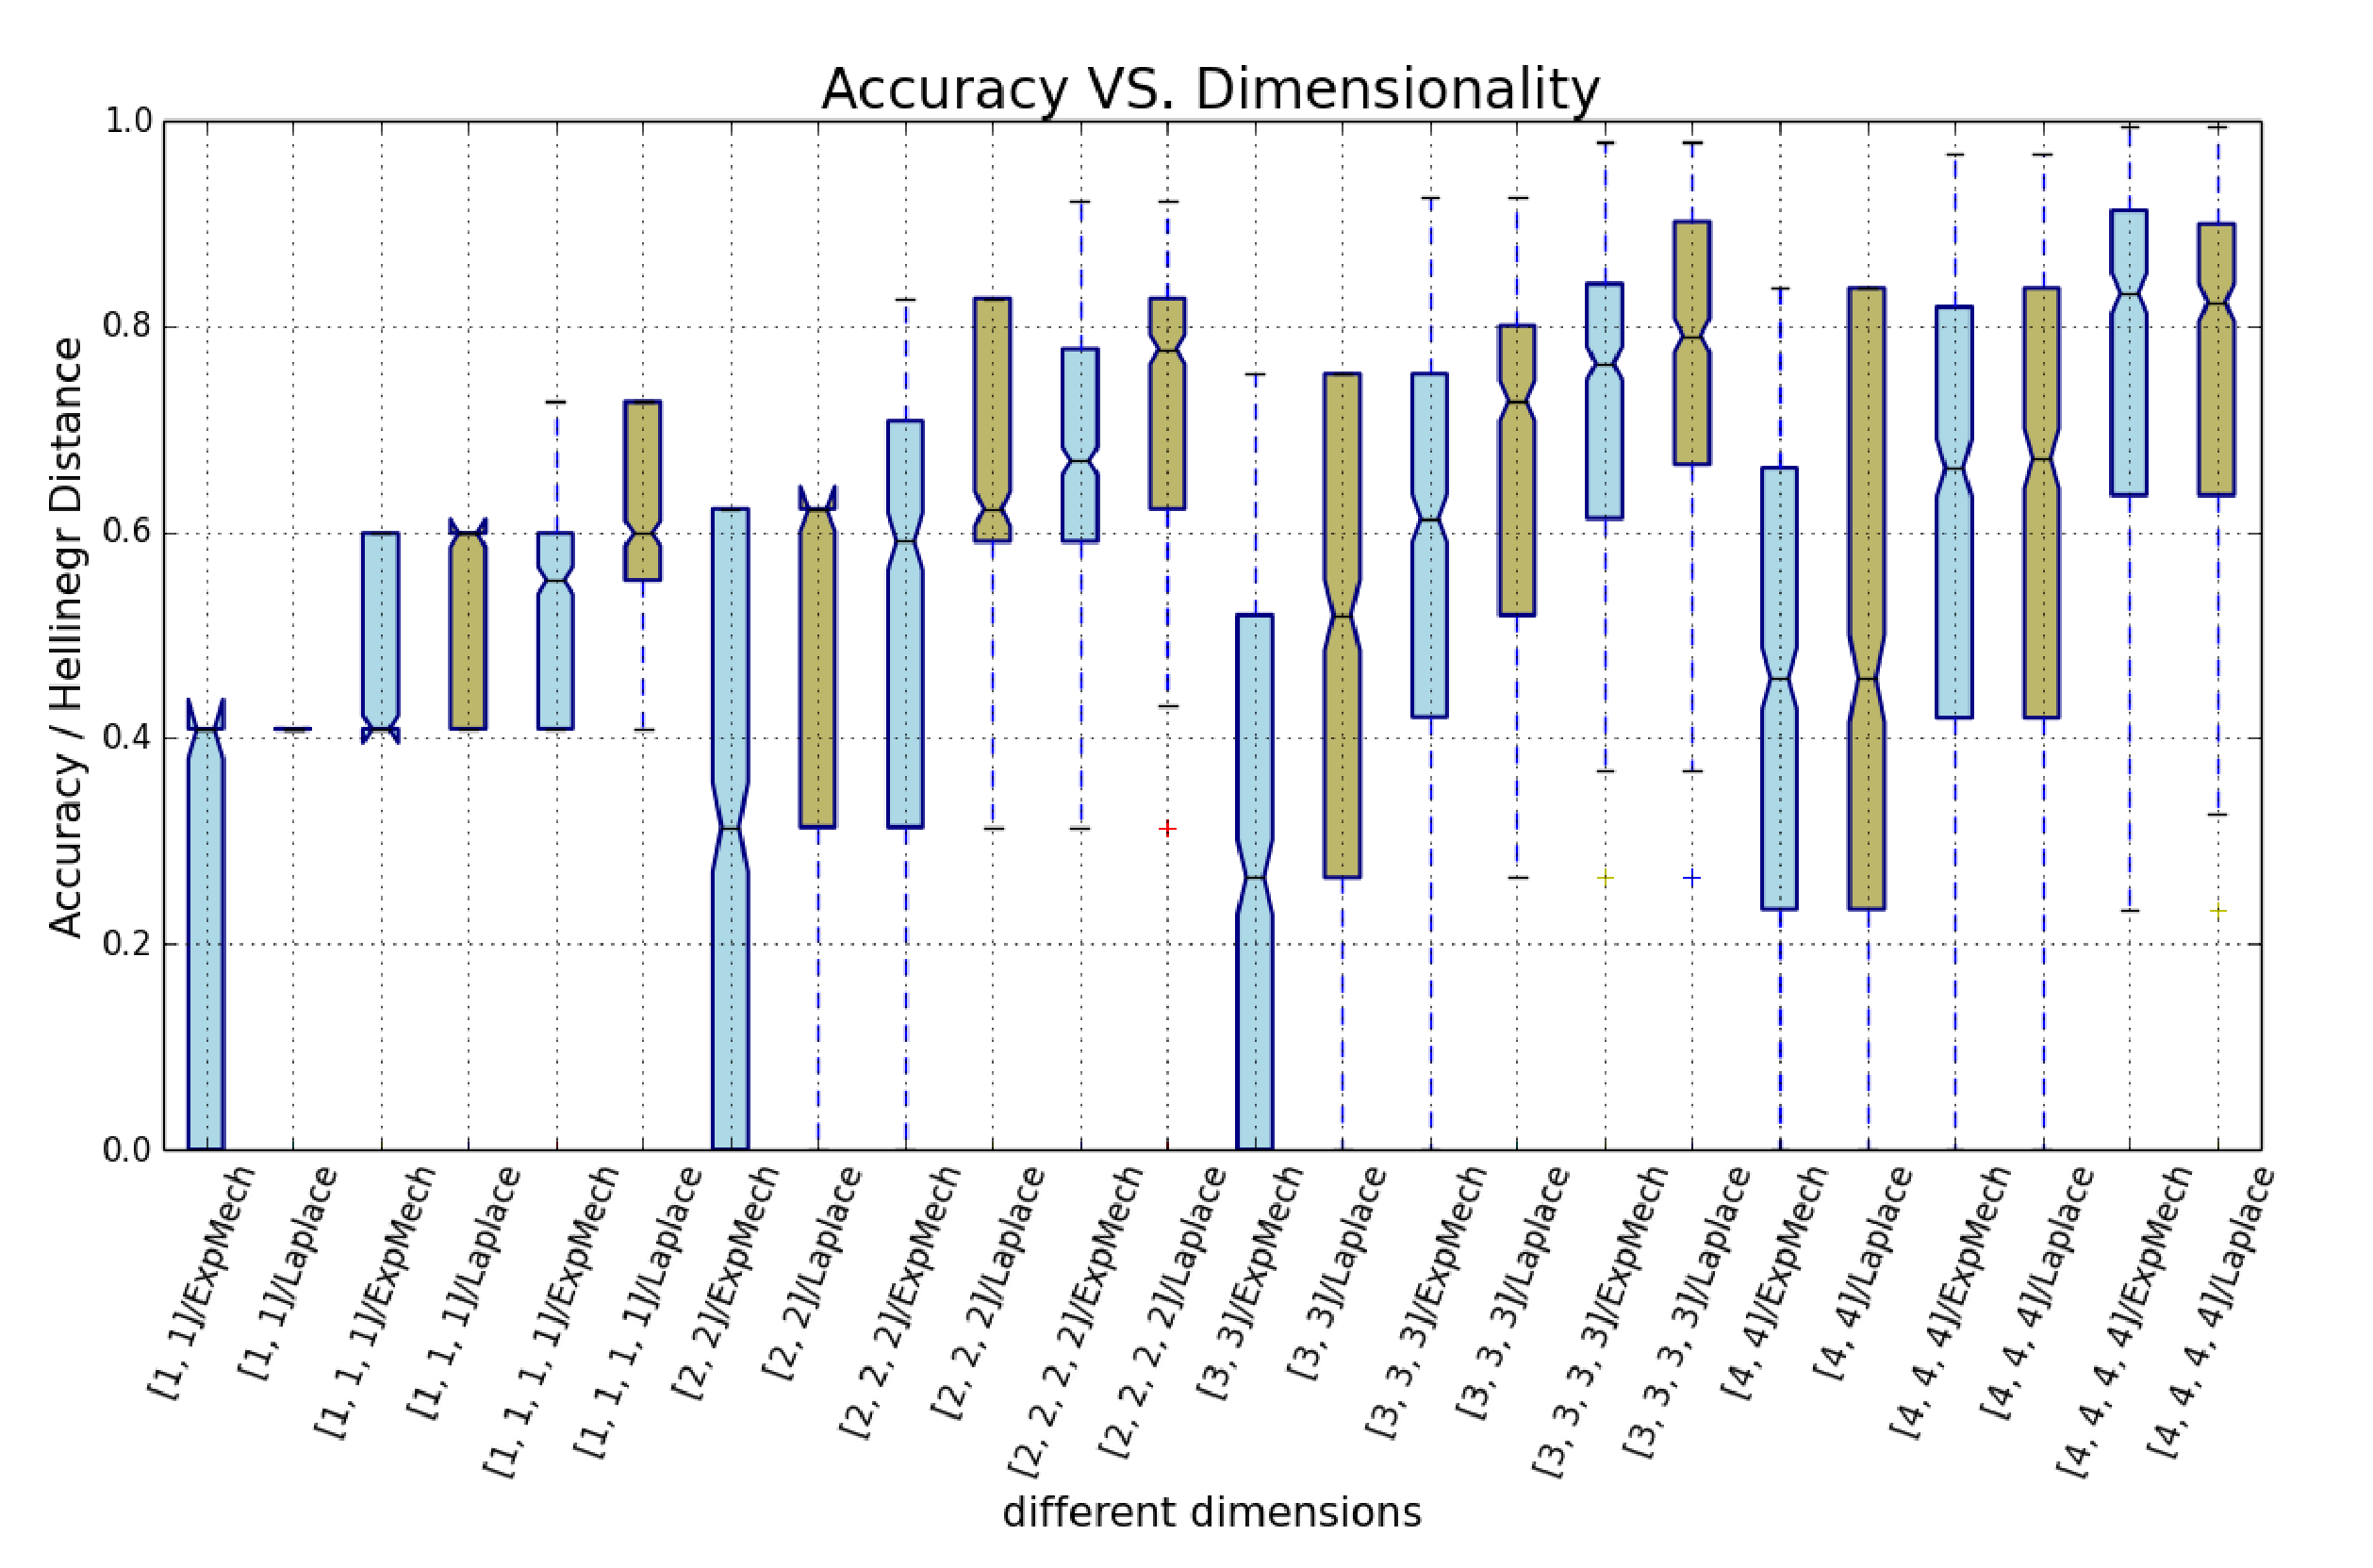
\includegraphics[width=1.0\textwidth]{accuracy_vs_dimension}
\caption{Accuracy measurement based on Hellinger distance wrt. different dimensions and data size. Settings: observed data are uniformly distributed, $\epsilon = 0.8$ and $\delta = 0.0005$, prior distributions are all $1$ in every dimension}
\label{fig_vs_dimension}
\end{figure}

In Fig. \ref{fig_vs_dimension}, x-axis are observed data sets of different size and dimensions. The plot shows that dimensions have similar influence on our exponential mechanism and the Laplace mechanism. Accuracy of two mechanisms both decrease when dimensions go larger. We will be beat by Laplace mechanism when data size increase but will not be affected when dimensions increase. In other words, dimension has little influence on whether we will beat Laplace mechanism.


\subsubsection{Accuracy Evaluation wrt. Data variance}
\label{subsubsec_vs_variance}

\begin{figure}[h]
\centering
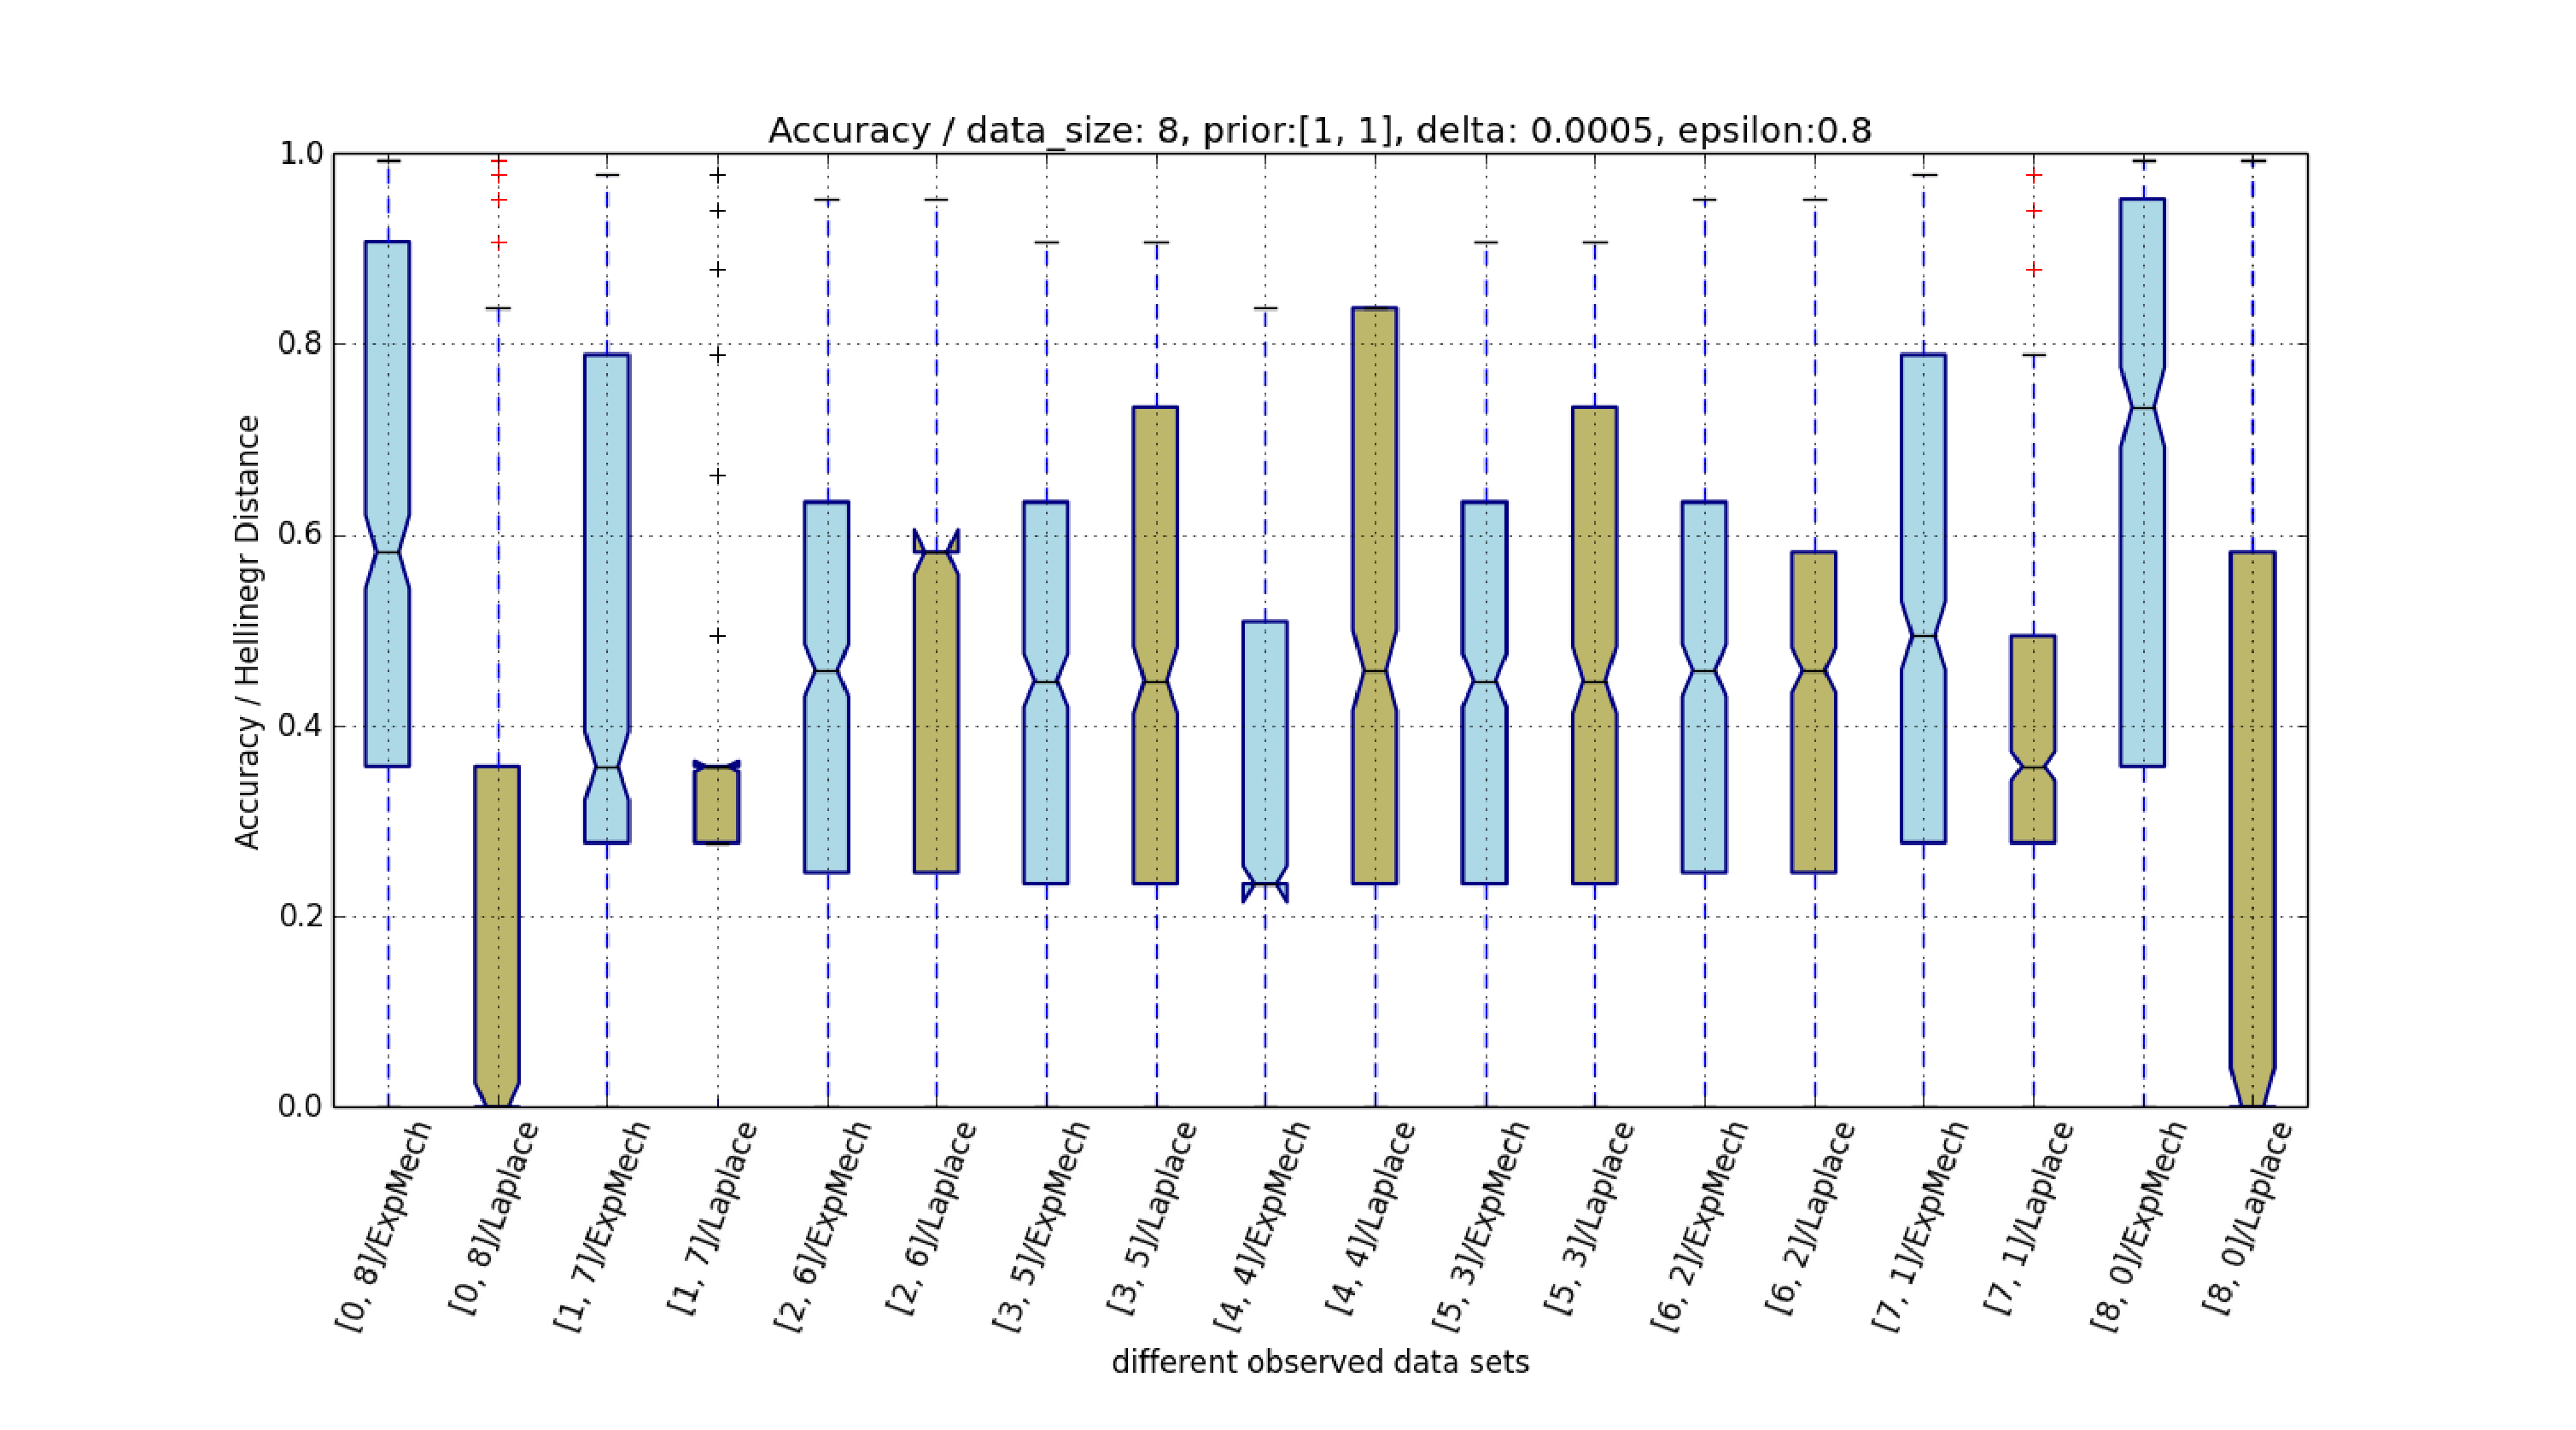
\includegraphics[width=1.0\textwidth]{accuracy_vs_mean_1_1}
\caption{Accuracy measurement based on Hellinger distance wrt. different data variance. Settings: $\epsilon = 0.8$ and $\delta = 0.0005$, prior distributions are all $1$ in every dimension}
\label{fig_vs_variance}
\end{figure}

In Fig. \ref{fig_vs_variance}, x-axis are observed data sets of different variances (or means). We study this variable under two-dimension $\betad$ distribution in order to be concise. It shows that our mechanism's accuracy is better when data variance go smaller, meanwhile Laplace mechanism go worse. We will beat Laplace mechanism when observed data are more uniformly.



\subsubsection{Accuracy Evaluation wrt. Prior Distribution}
\label{subsubsec_vs_prior}

\begin{figure}[h]
\centering
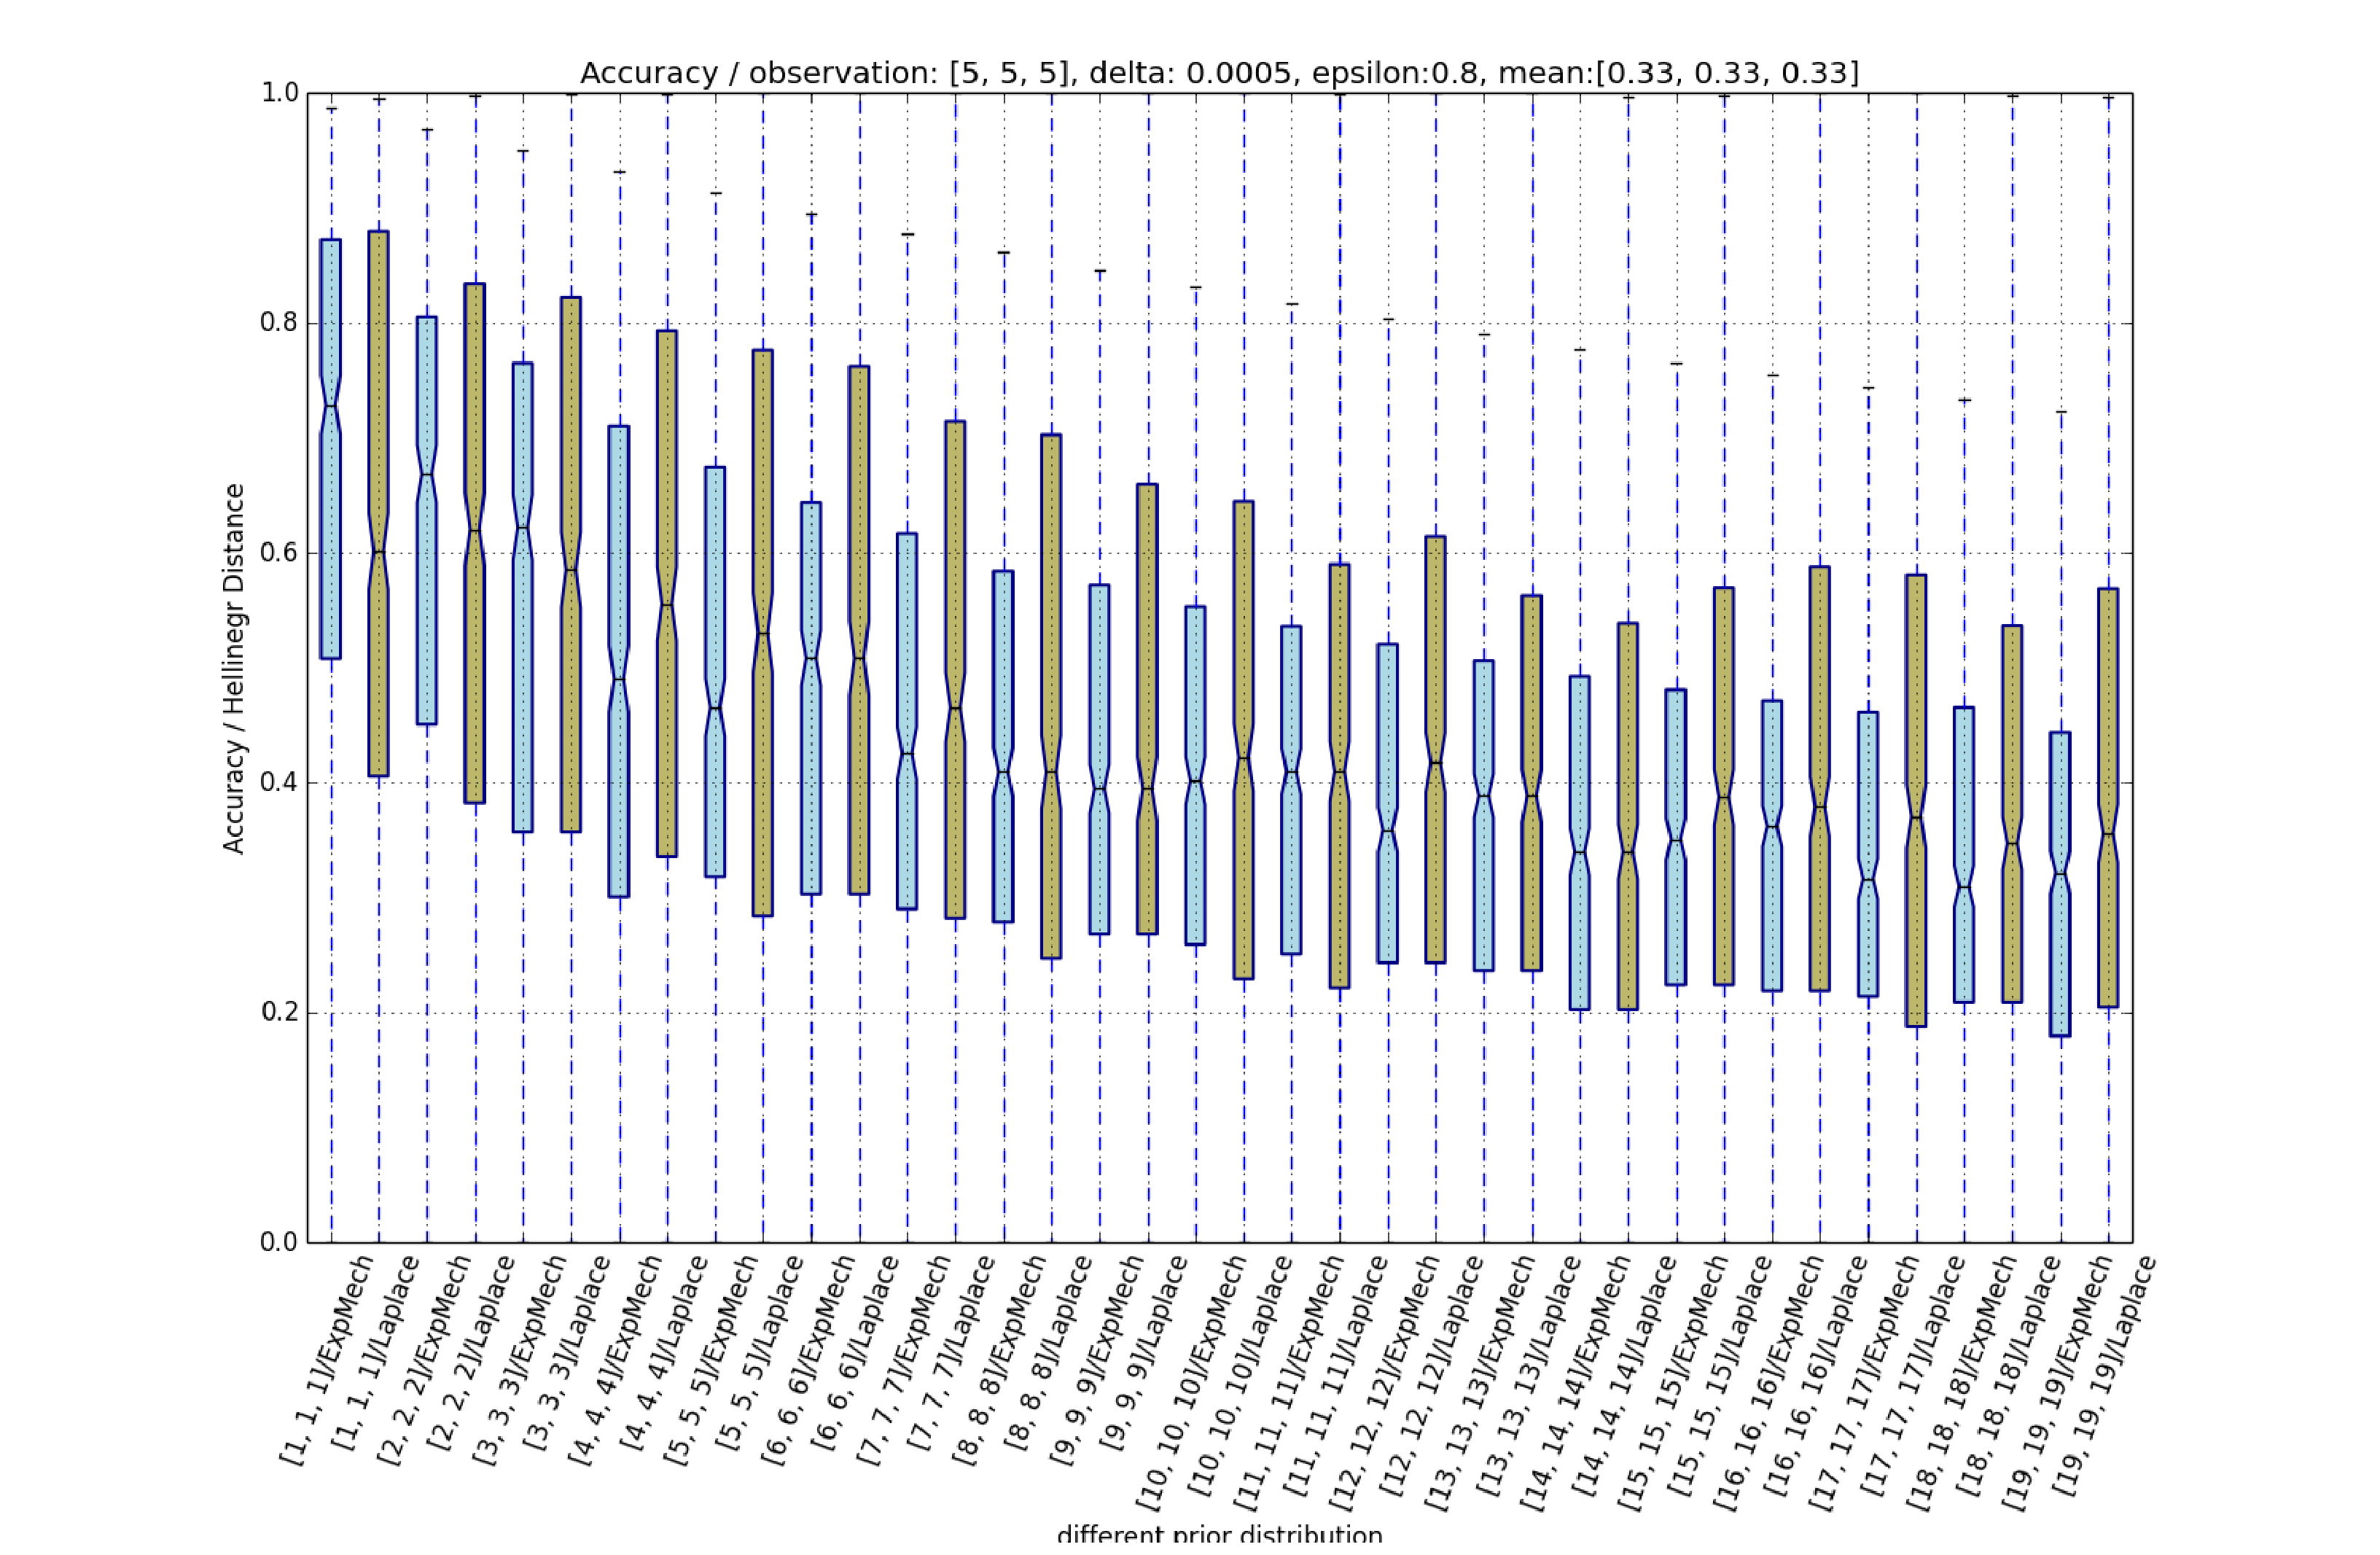
\includegraphics[width=1.0\textwidth]{accuracy_vs_prior_5_5_5}
\caption{Accuracy measurement based on Hellinger distance wrt. different prior distribution. Settings: $\epsilon = 0.8$ and $\delta = 0.0005$, observed data set is: $[5,5,5]$}
\label{fig_vs_prior}
\end{figure}

In Fig. \ref{fig_vs_prior}, we study this variable under setting that observed data set is $[5,5,5]$ because in Fig. \ref{fig_vs_datasize} Laplace mechanism beat us when data size is 15 and uniformly distributed.





\subsubsection{Accuracy Evaluation wrt. Prior Distribution and Data Variance}
\label{subsec_vs_prior_variance}

\begin{figure}[h]
\centering
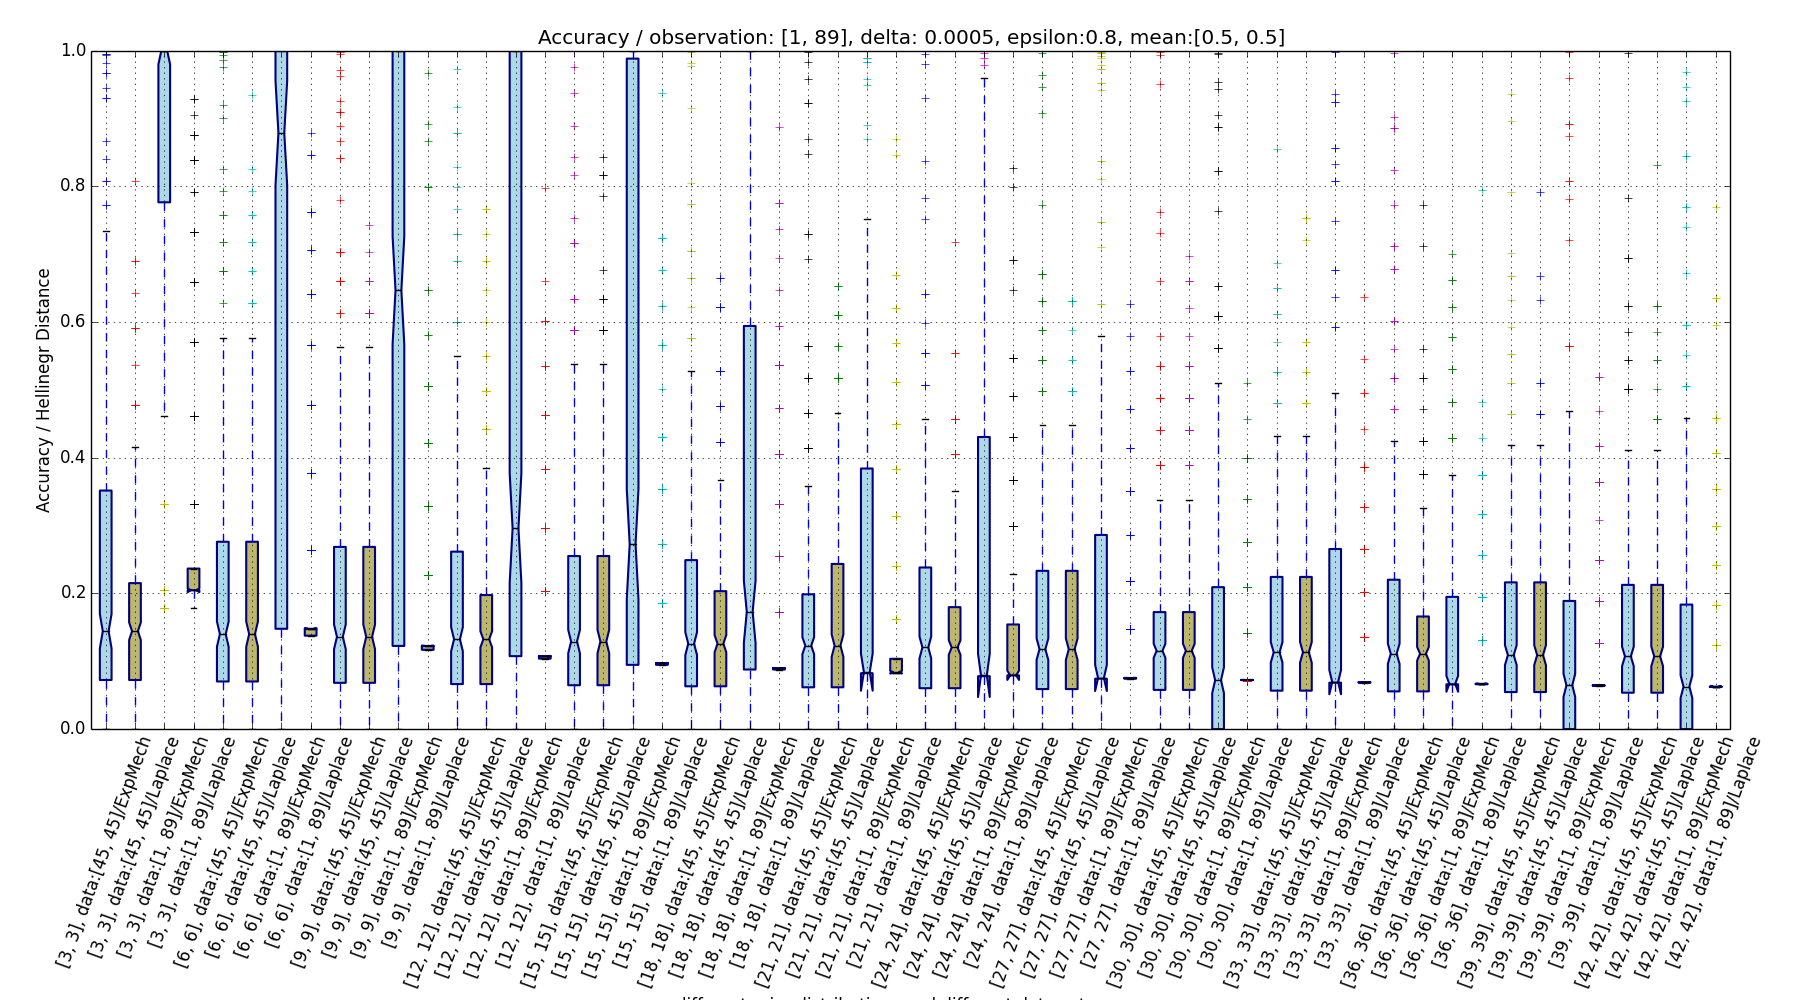
\includegraphics[width=1.0\textwidth]{Accuracy_VS_Prior_mean}
\caption{Experimental Results for Finding the Local Sensitivity Efficiently}
\label{fig_vs_prior_variance}
\end{figure}

\subsection{Experiment Evaluations on Privacy}
\label{subsec_experiment_privacy}
In order to see our privacy behavior, we study the accurate epsilon under concrete cases in this section. The $(\epsilon, \delta)$ - differential privacy we proved in Sec. \ref{sec_smoo} is just an upper bound, we concrete $\epsilon$ should be smaller than upper bound in our exponential mechanism. We calculate the concrete privacy value in following ways wrt. the data size, and obtain plots in Fig. \ref{fig_privacy}.

\begin{figure*}
\begin{center}
\centering
  \subfigure[data size range from 90 to 180]{
    \includegraphics[width=0.48\textwidth]{global_epsilon_20_20.eps}}
  \subfigure[data size range from 90 to 180]{
    \includegraphics[width=0.48\textwidth]{global_epsilon_20_20(2).eps}} 
\caption{Concrete privacy calculation under settings that: prior distribution:$[1,1]$, $\epsilon = 0.8$, $\delta = 0.0005$ and observed data are uniformly distributed}
\label{fig_privacy}
\end{center}
\end{figure*}

$\epsilon = $


\bibliographystyle{plain}
\bibliography{bayesian.bib}

\end{document}

